\documentclass[xcolor=table,aspectratio=169]{beamer}

\usepackage{presentation}



\usetheme{ift}




% % % % Title page % % % % % % % % % % % % \centerline{presentation}

\title{Quantum Chemical and Molecular Dynamics Synergism: Study of 2D Materials and Polymer Matrices} 
\subtitle{}

\author{Speaker: Le Nhan Pham}
\institute{College of Science and Engineering - Flinders Uni - Australia}
\date{\today} 


% % % % End of title page % % % % % % % % % % % %
\DeclareUnicodeCharacter{2212}{-}

\begin{document}

\begin{frame}
	\titlepage
\end{frame}





% Outline or Table of contents
\begin{frame}{Outline} %%[allowframebreaks]
	\frametitle{Outline}
	\tableofcontents
\end{frame}

% % % spreading line % % % %

\linespread{1.5}

% % % Contents of the presentation % % % %


\section{Introduction}

\begin{frame}{Factors affect decision on the choice of levels of theory}
	\begin{columns}
		\begin{column}{0.55\textwidth}
			\begin{itemize}
				\item Factors that affect the choice of theory levels
				      \begin{itemize}
					      \item Sizes of the studied systems
					      \item Properties that we want to study
					      \item Available computational resources
					      \item Availability of well tested theoretical methods
				      \end{itemize}
			\end{itemize}
		\end{column}
		\begin{column}{0.45\textwidth}
			\begin{figure}
				\centering
				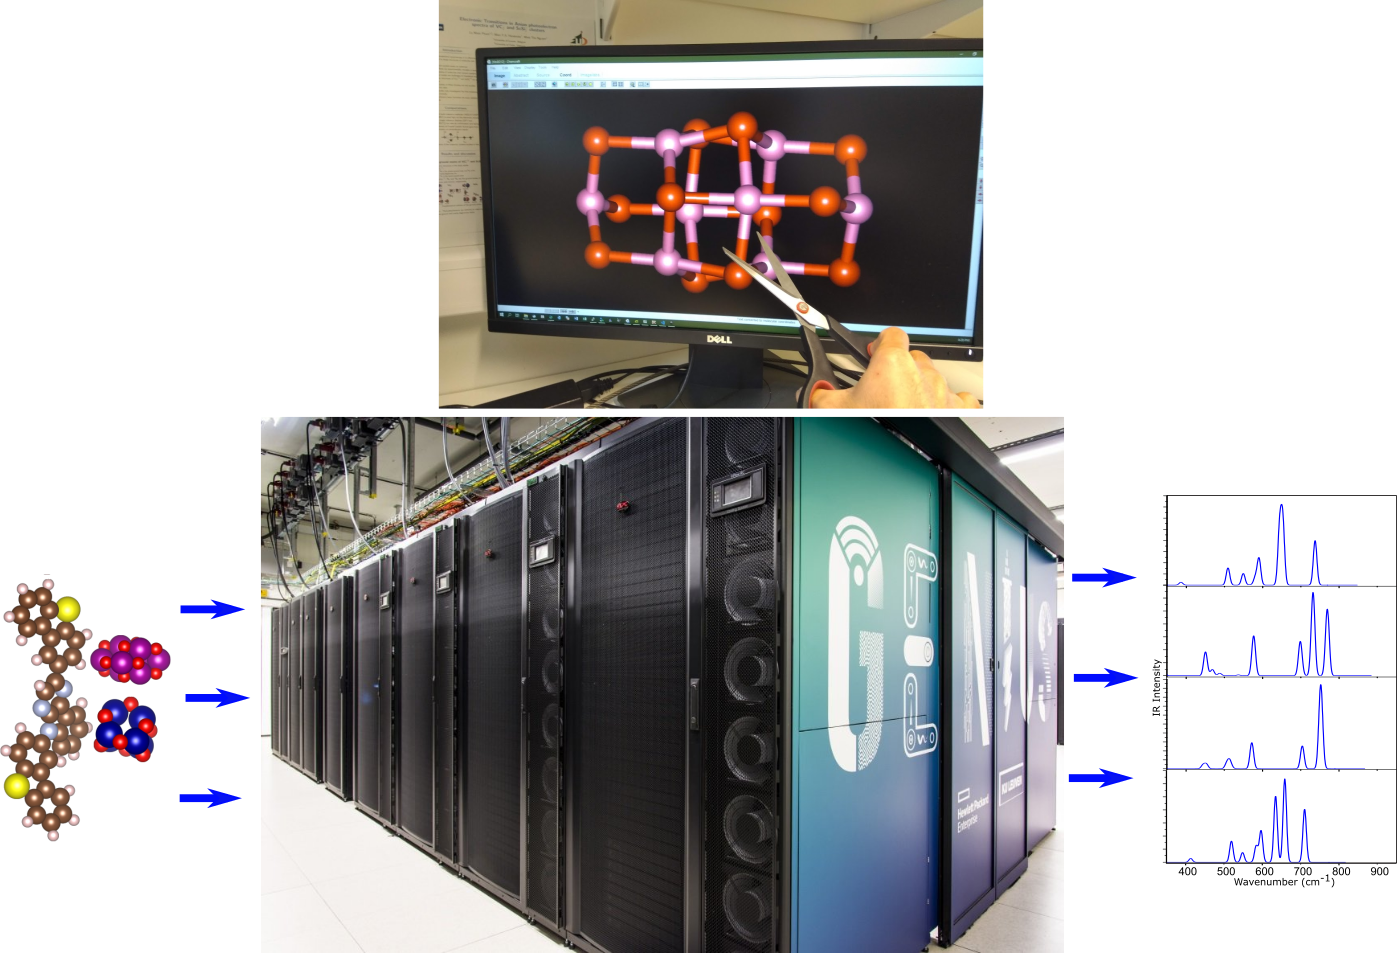
\includegraphics[width=0.9\textwidth]{systems-properties-resources}
			\end{figure}
		\end{column}
	\end{columns}
\end{frame}


\begin{frame}
	\frametitle{Computational/Chemical methods}
	\begin{figure}
		\centering
		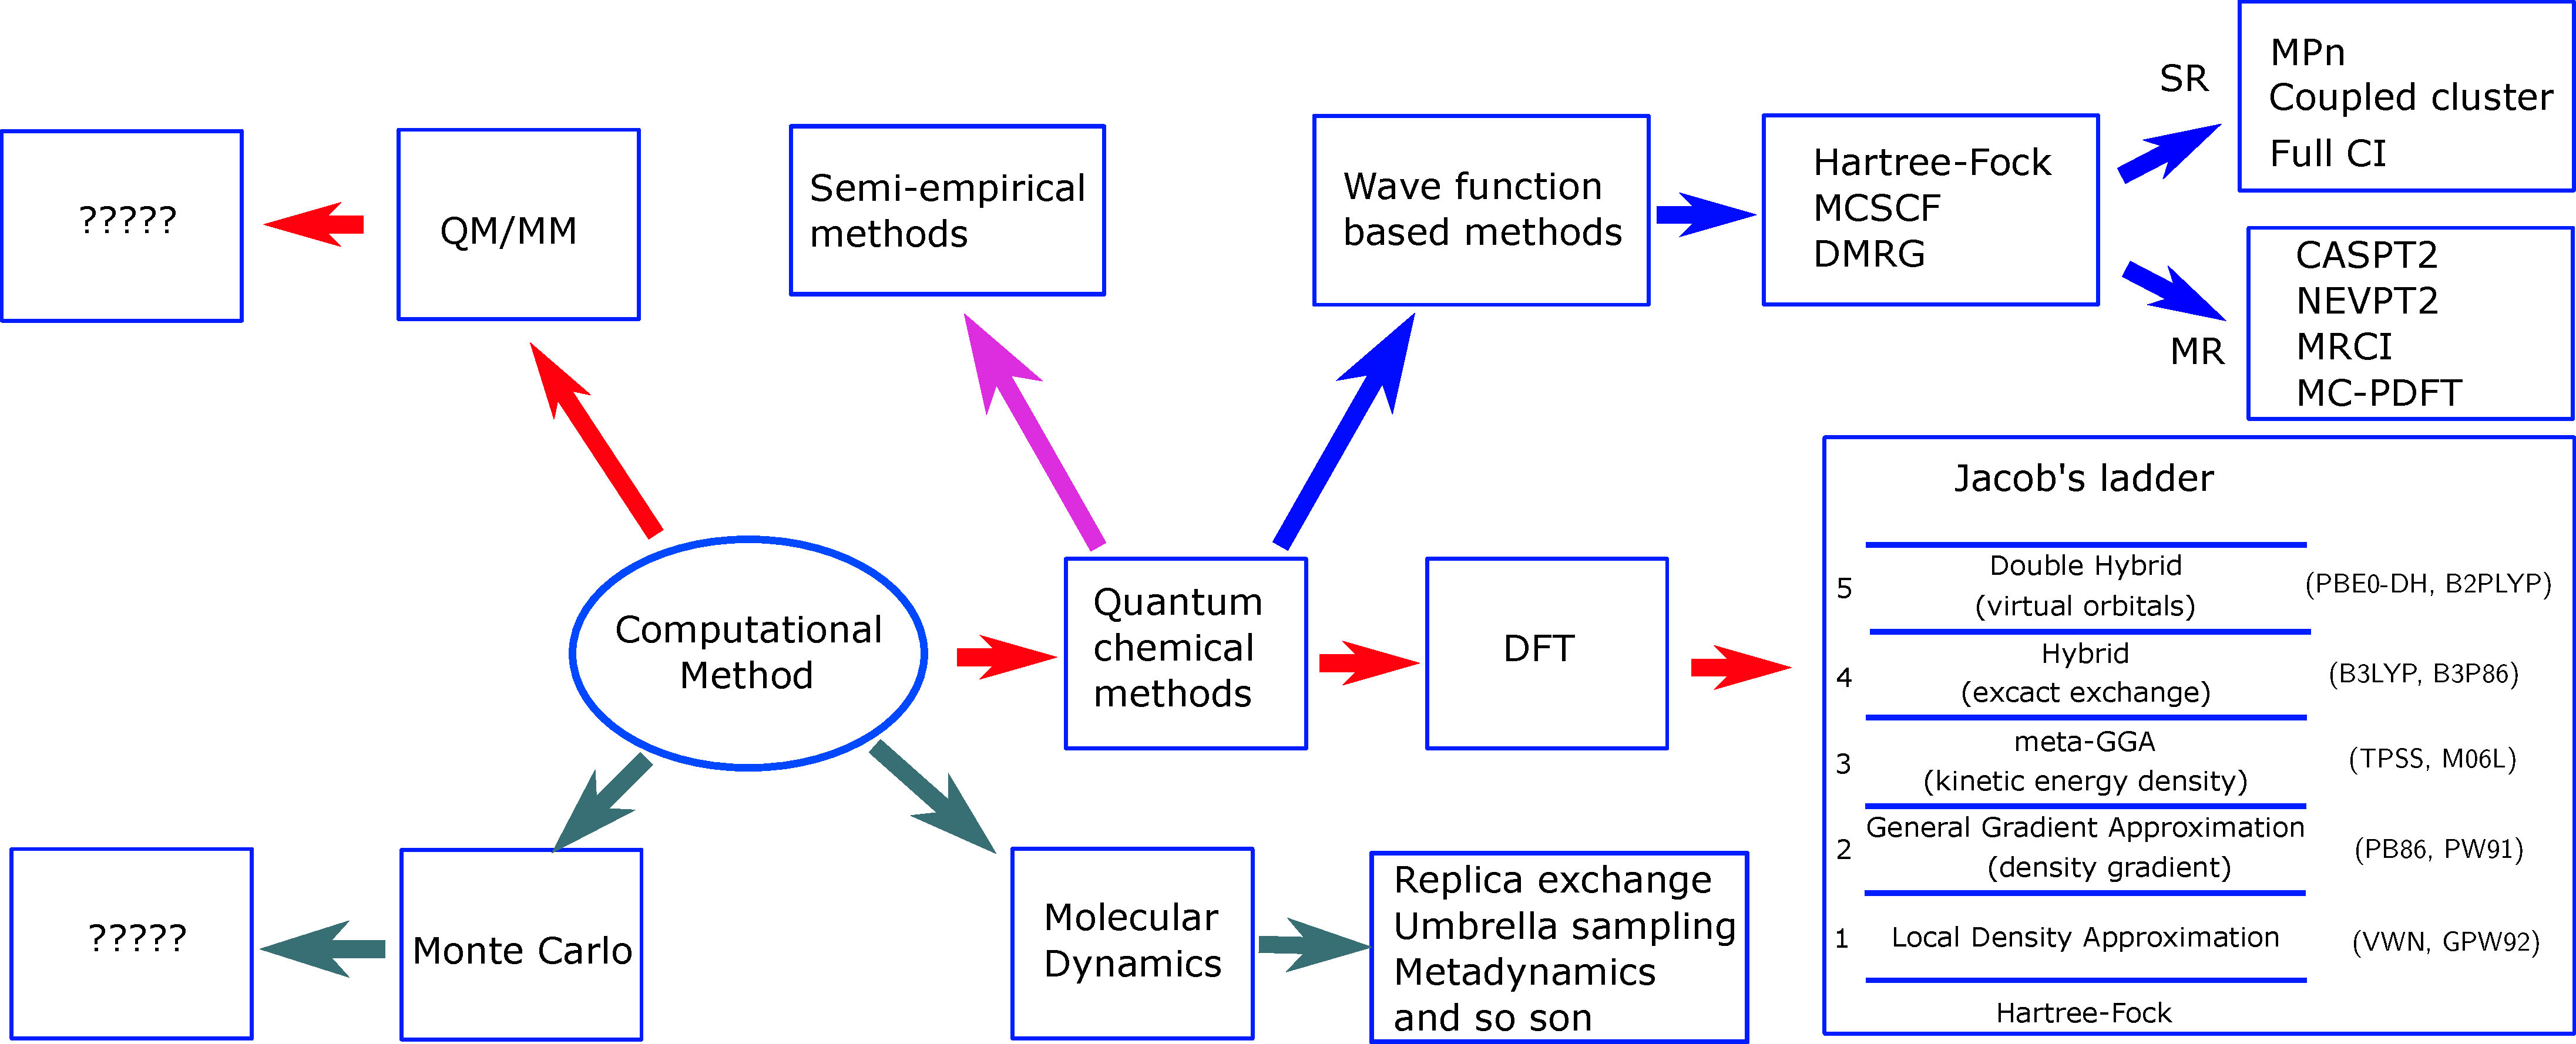
\includegraphics[width=\textwidth]{computational-methods}
	\end{figure}
\end{frame}


\begin{frame}
	\frametitle{In this talk}

	\begin{itemize}
		\item Talk about the synergism between QM and MM in study of complicated chemical systems
		      \begin{itemize}
			      \item Use quantum chemical data to \textcolor{blue}{revisit, benchmark, and develop} force fields for big systems
			      \item As an example, \textcolor{blue}{develop a totally new force field} for simulations of biomolecules on the surface of a 2D surface (\ch{MoS2})
			      \item \textcolor{blue}{Employment of MD techniques to construct complicated systems} for further quantum chemical computations: 3D crosslinked polymer matrices
		      \end{itemize}
	\end{itemize}

\end{frame}


\section[Development of an MD force field]{Development of an MD force field for simulations of 2D \ch{MoS2-H2O} interaction}


\begin{frame}
	\frametitle{2D \ch{MoS2} and exfoliation}
	\begin{columns}
		\begin{column}{0.7\textwidth}
			\begin{itemize}
				\item \textcolor{blue}{Wide range of potential applications of 2D \ch{MoS2}}: biosensing, gas sensing, water purification, drug delivery, electronic devices
				\item \textcolor{blue}{Production of 2D materials including \ch{MoS2}}: Exfoliation using organic solvents and biomolecules (peptides)
				\item \textcolor{blue}{To study the exfoliation process theoretically}: Develop a FF to accurately capture interaction between 2D \ch{MoS2} and absorbents
			\end{itemize}
		\end{column}
		\begin{column}{0.4\textwidth}
			\begin{figure}
				\centering
				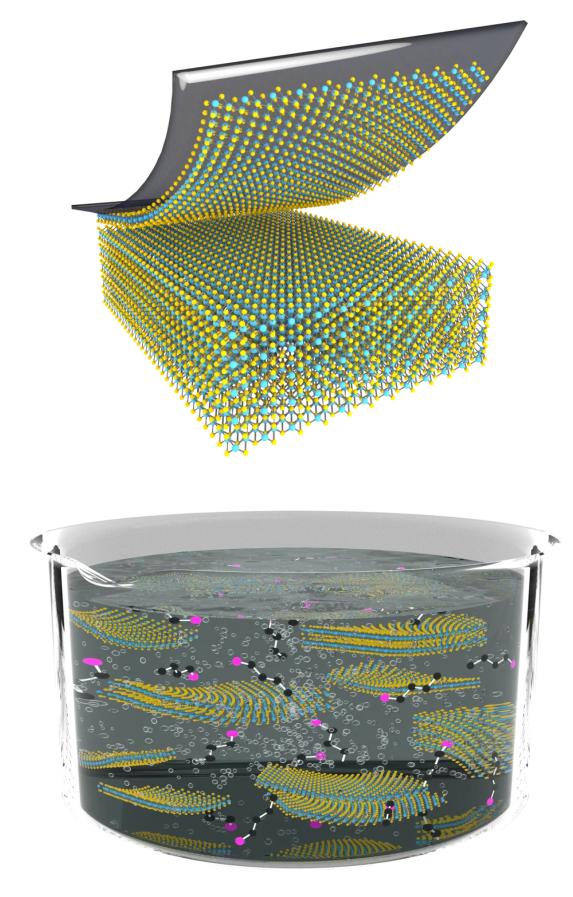
\includegraphics[height=0.7\textheight]{exfoliation-MoS2}
			\end{figure}
		\end{column}
	\end{columns}
	\hfill \tiny{the image was taken from www.ossila.com}
\end{frame}



\begin{frame}
	\frametitle{Revisit and benchmark available force fields before use: \ch{MoS2}}
	\textcolor{blue}{Several FFs available for simulations of interaction between 2D \ch{MoS2} and \ch{H2O}:}
	\begin{tikzpicture}[overlay]
		\node[inner sep=0pt] (contactAngle) at (1,-1.65)
		{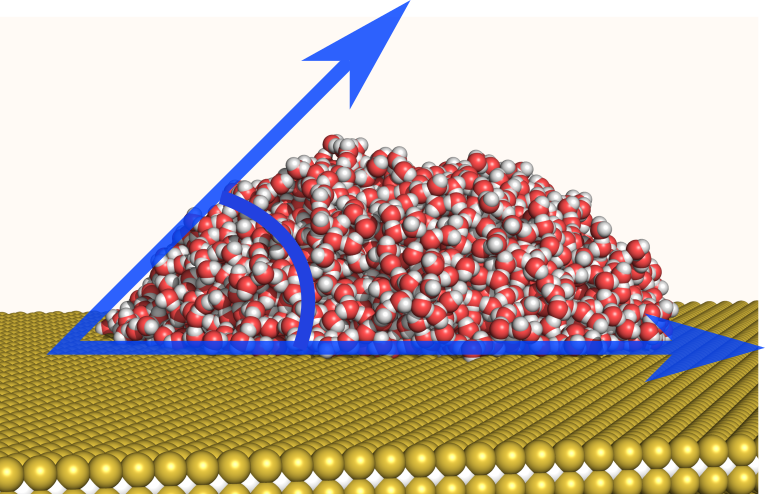
\includegraphics[width=.15\textwidth]{contact-angle}};
	\end{tikzpicture}
	\begin{itemize}
		\item Can reproduce experimental macroscopic features of water on \ch{MoS2}: water contact angle
		\item They cannot correctly describe microscopic structures of water on \ch{MoS2}
	\end{itemize}
	\textcolor{red}{$\Rightarrow$ Introduce a new criterion: energetic ranking}
	\begin{figure}
		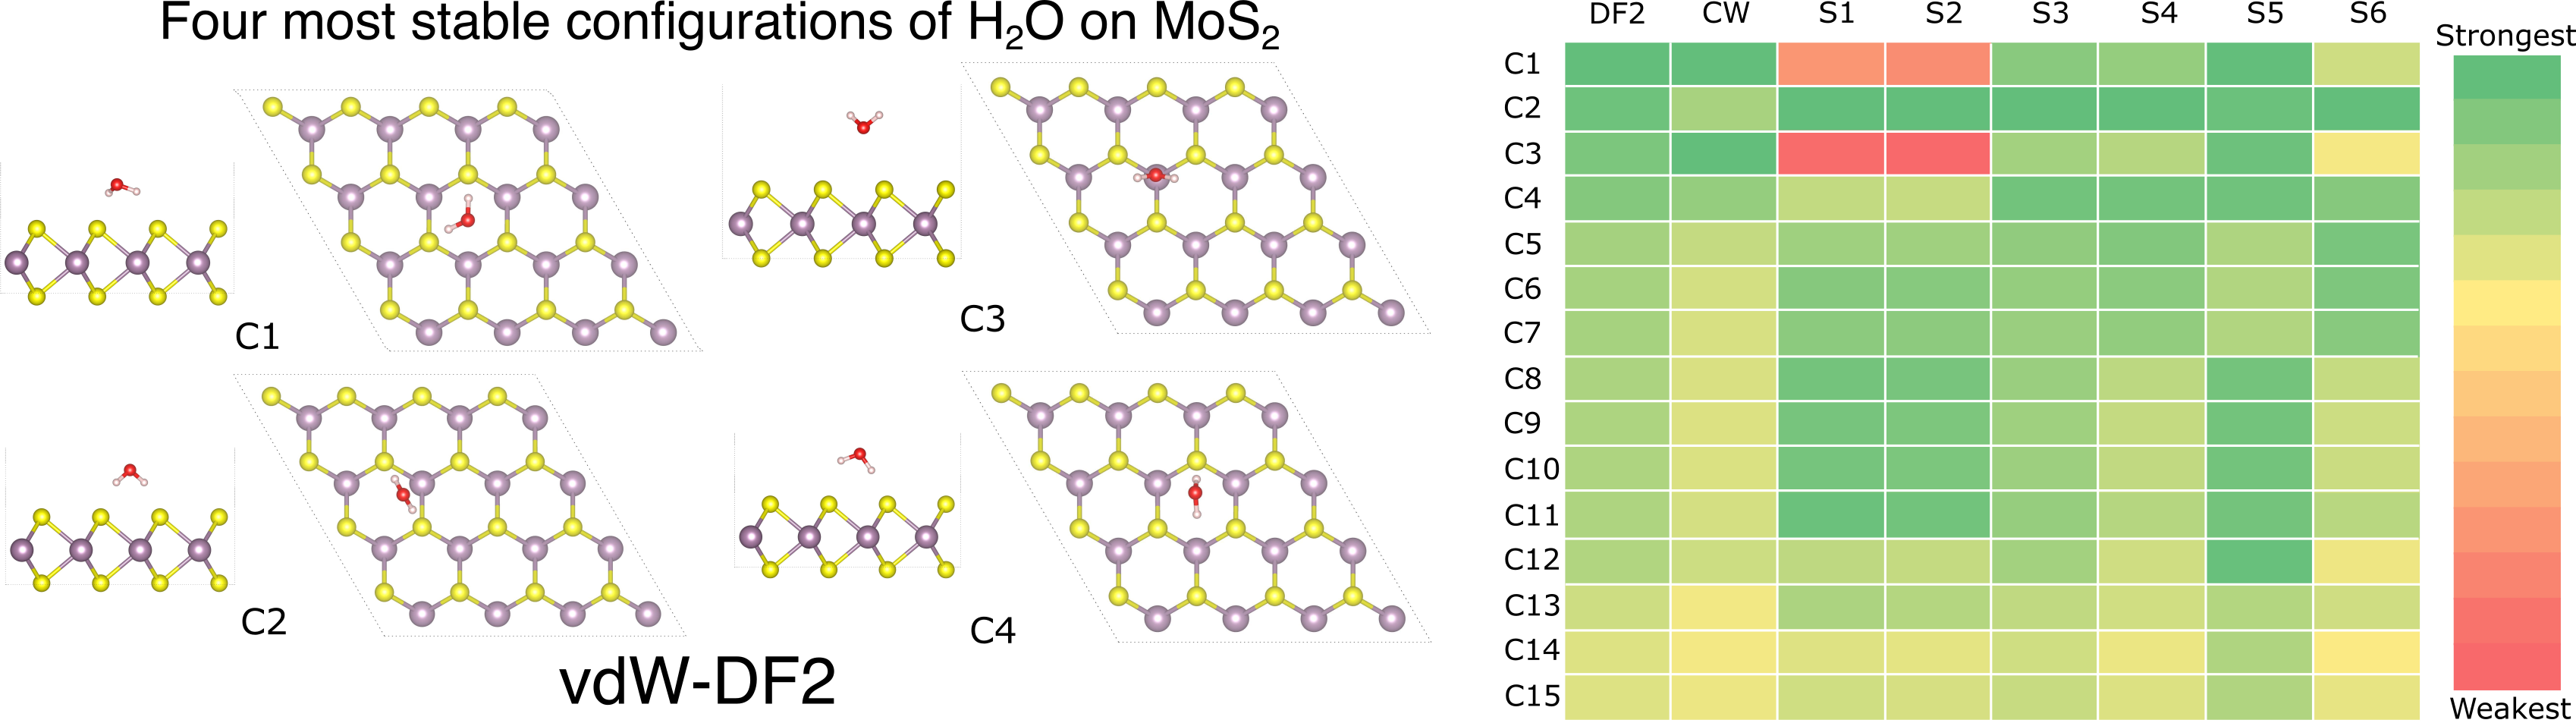
\includegraphics[width=0.95\textwidth]{MoS2-water-different-FFs}
	\end{figure}
\end{frame}


\begin{frame}
	\frametitle{Develop a new FF: \ch{MoS2-H2O} interaction}
	\textcolor{blue}{Developed a new set of FF parameters to \\ describe \ch{MoS2-H2O} interaction}
	\begin{columns}
		\begin{column}{0.6\textwidth}
			\vspace{-0.6cm}
			\begin{itemize}
				\item Reproduces contact angle of water on \ch{MoS2}
				\item Captures structural features of water on \ch{MoS2}
				\item Recovers QM energetic ranking of configurations
			\end{itemize}
			\vspace{-0.4cm}
			\begin{figure}
				\centering
				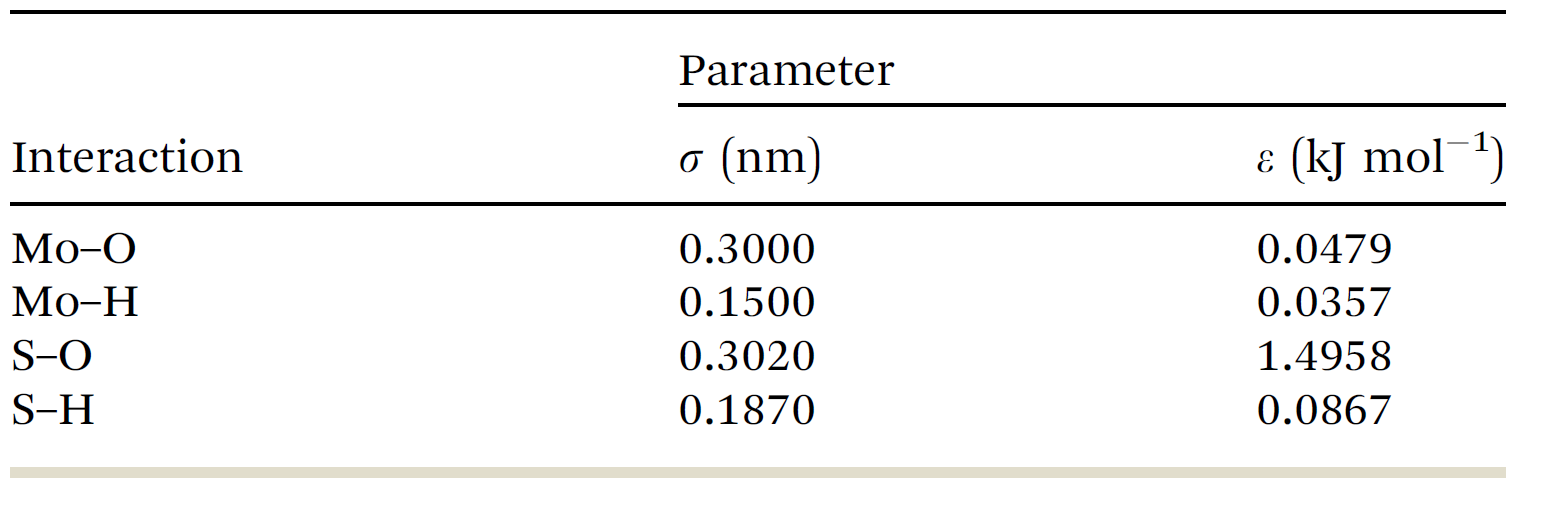
\includegraphics[width=0.9\textwidth]{MoS2-water-parameters}
			\end{figure}
		\end{column}
		\begin{column}{0.5\textwidth}
			\vspace{-1.4cm}
			\begin{figure}
				\centering
				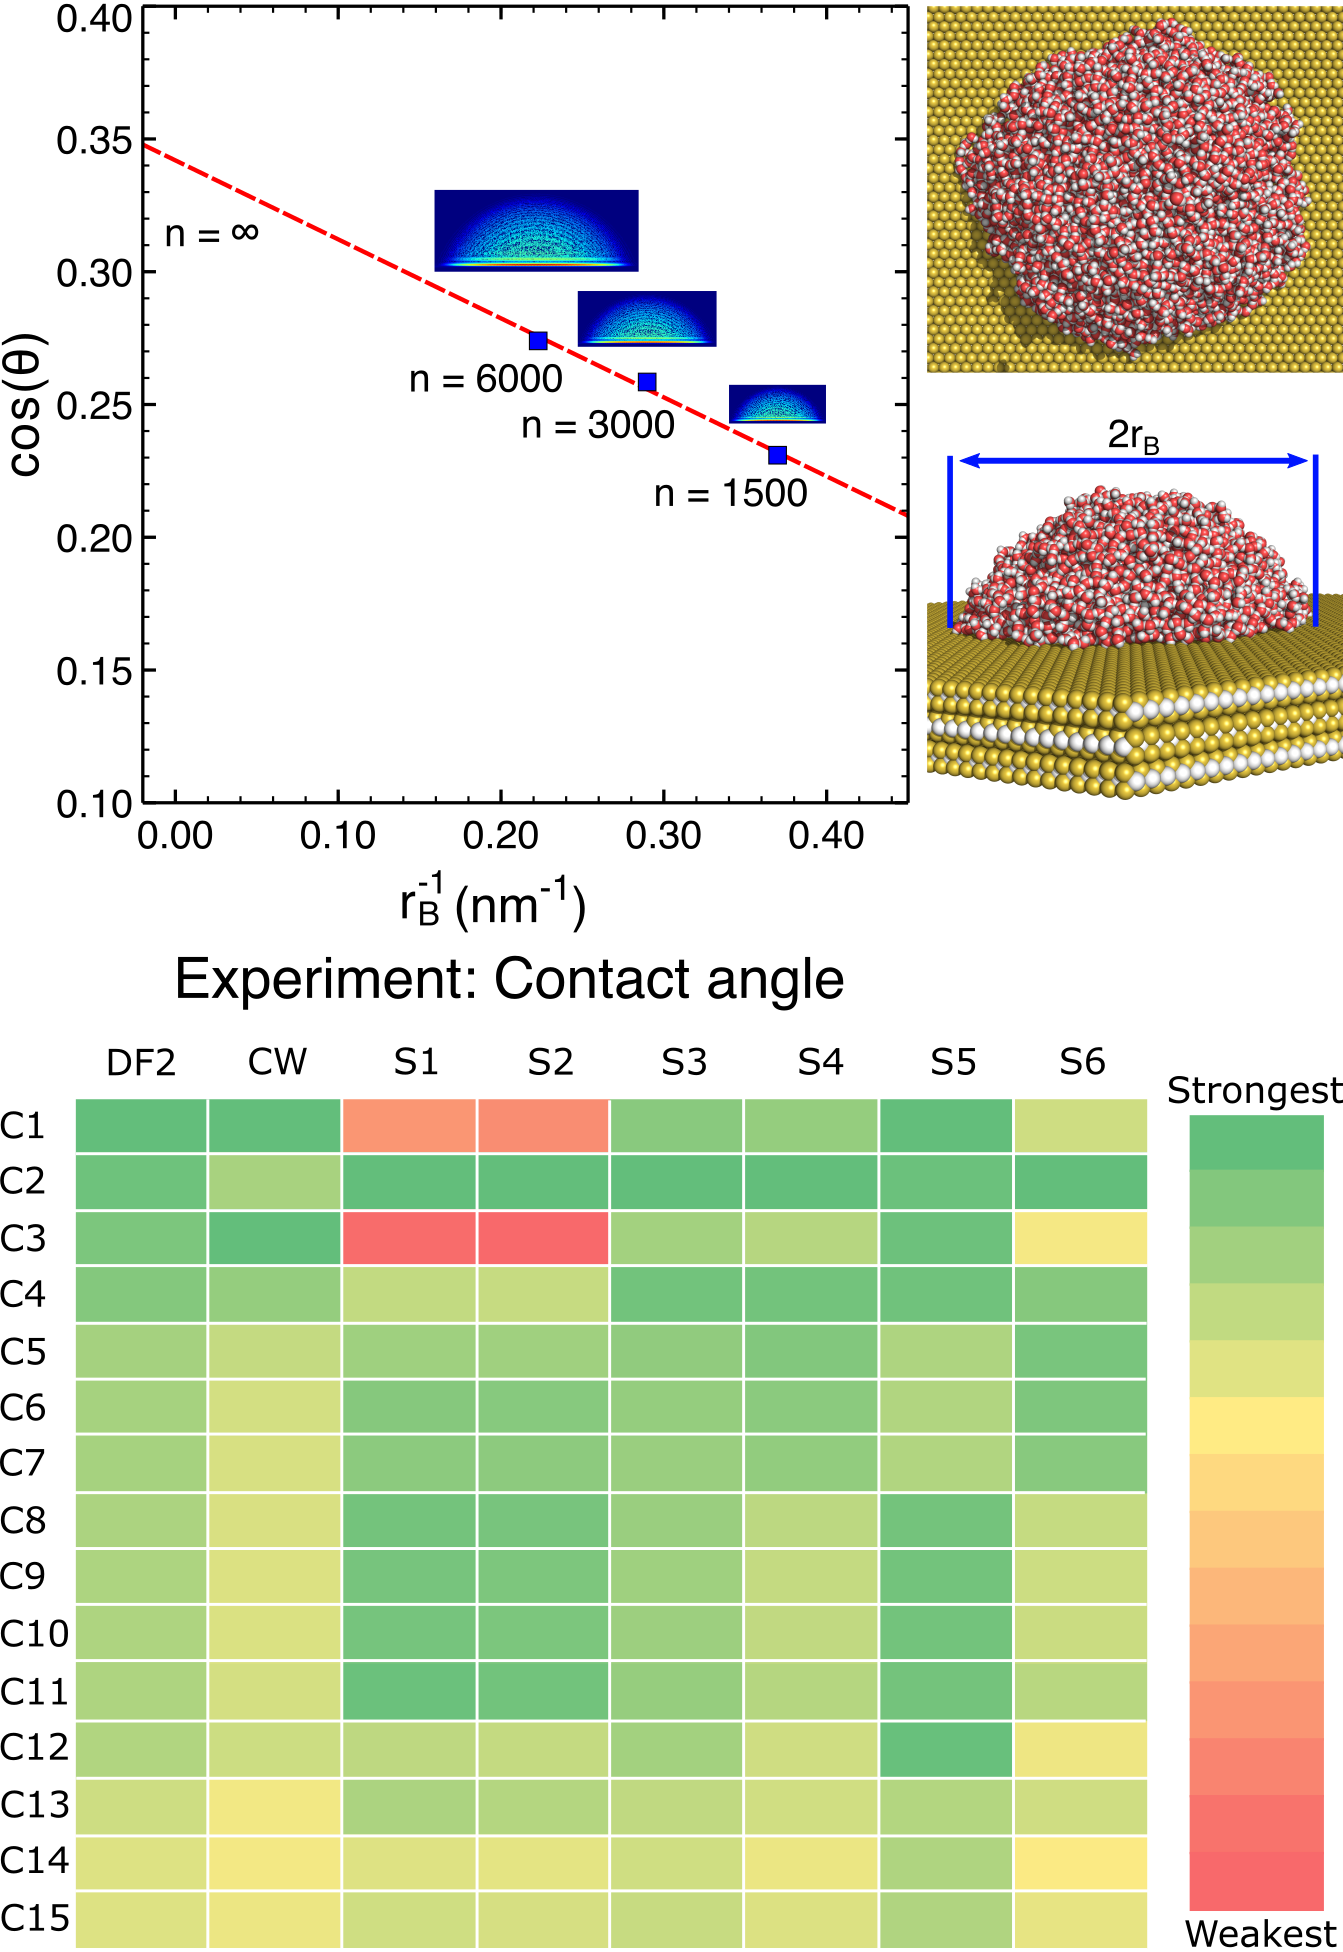
\includegraphics[height=0.88\textheight]{FF-MoS2-water}
			\end{figure}
		\end{column}
	\end{columns}
	\vspace{-0.4cm}
	\tiny{Pham, L. N.; Walsh, T. R. \emph{Chem. Commun.} 2021, 57 (27), 3355–3358}
\end{frame}


\begin{frame}
	\frametitle{Develop a new FF: \ch{MoS2-peptide} interaction}
	\begin{figure}
		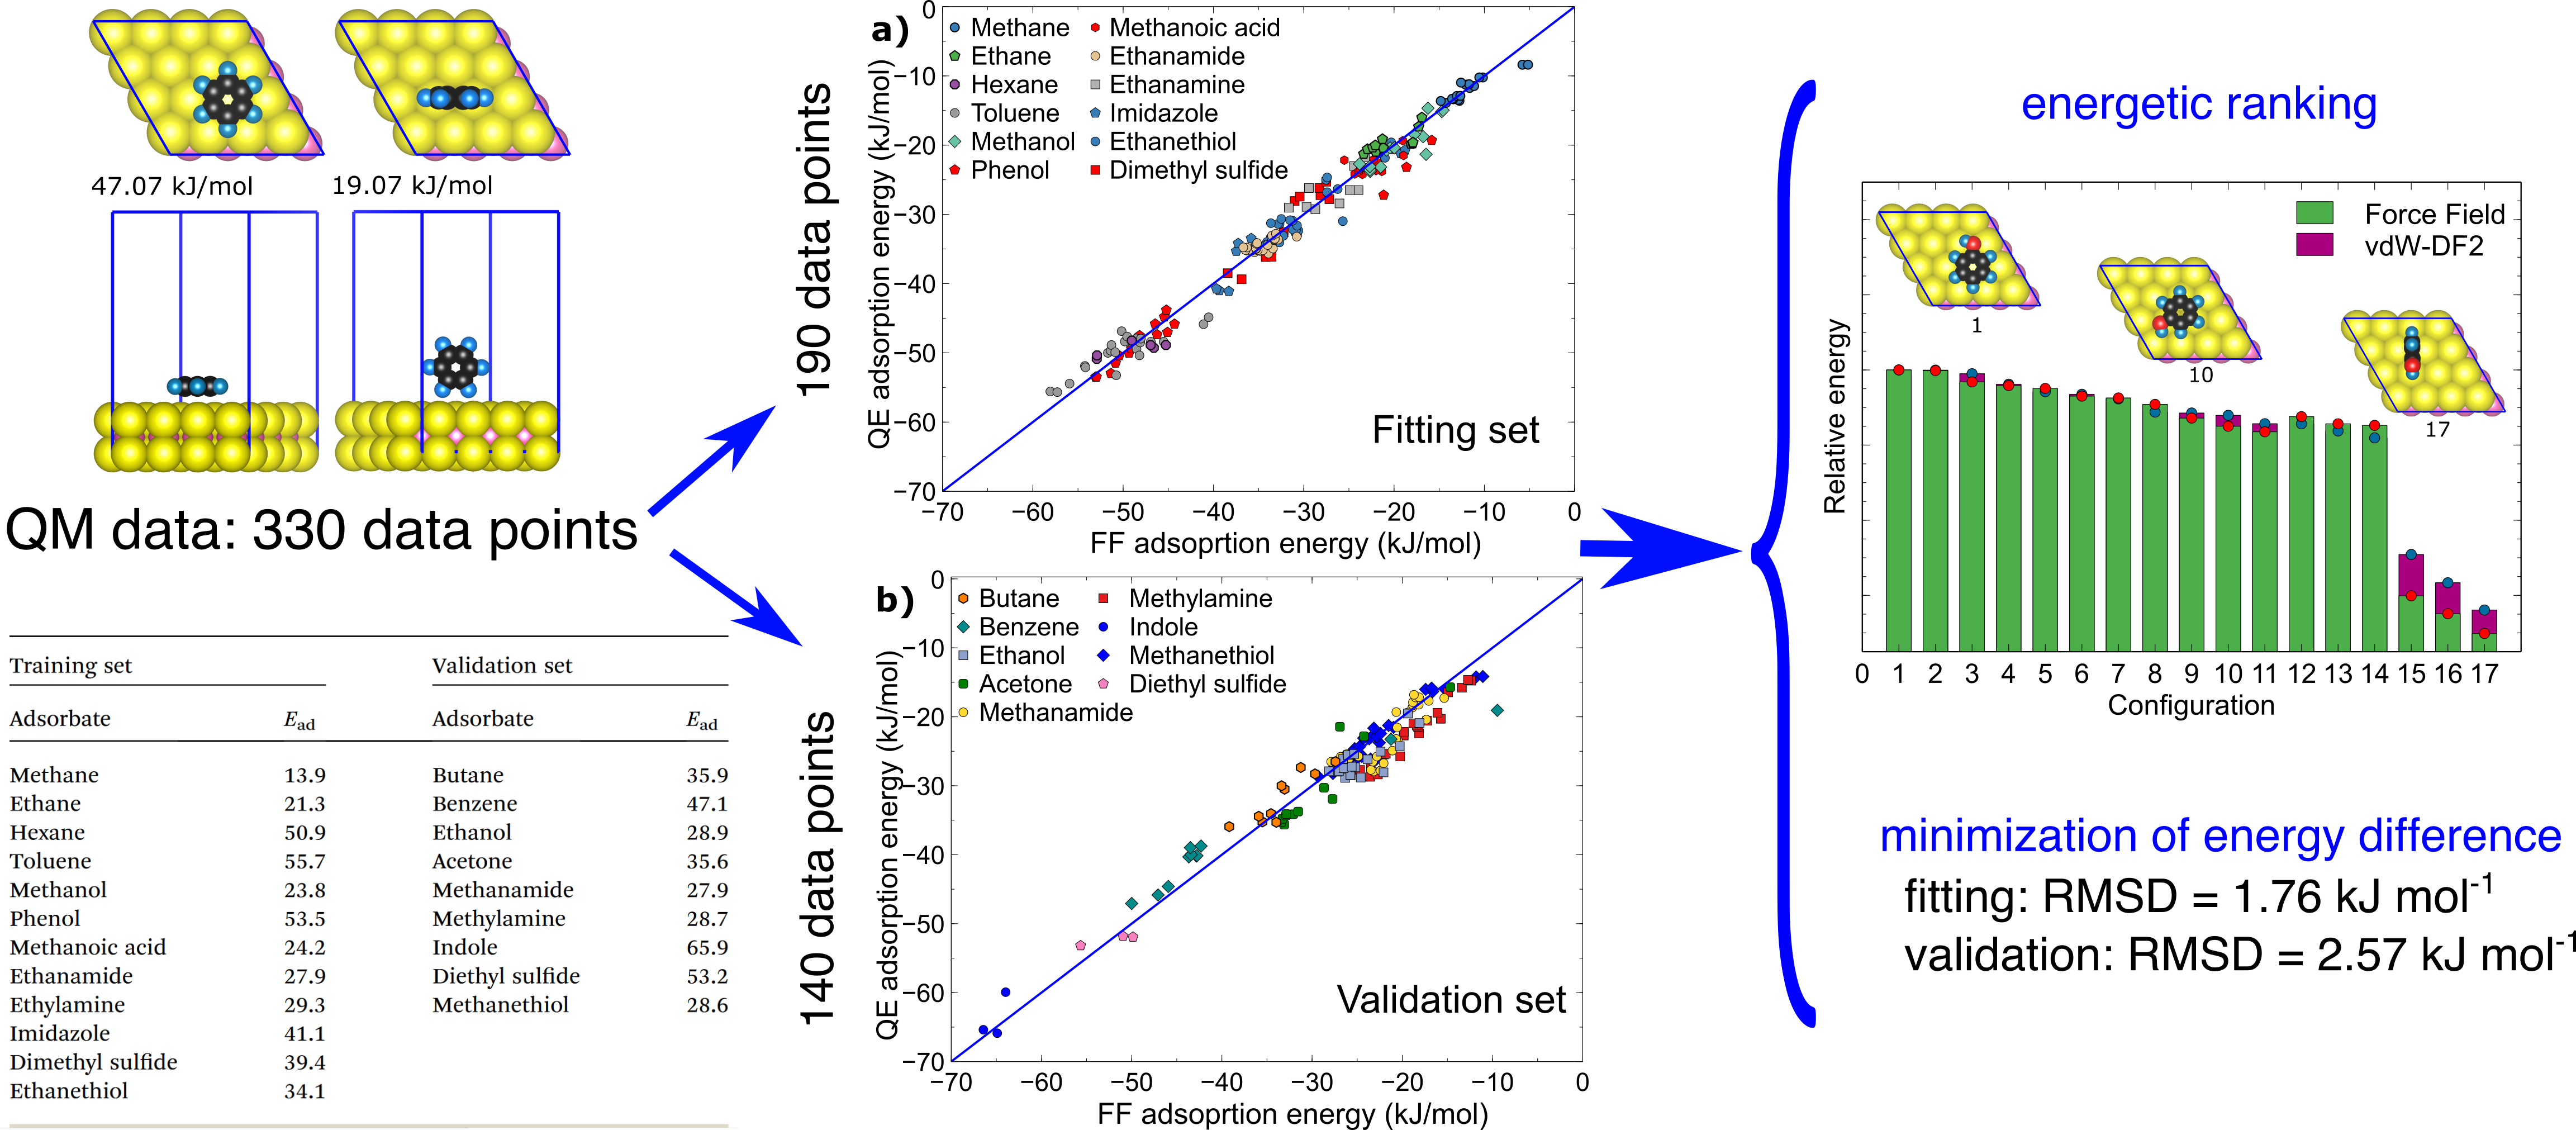
\includegraphics[width=\textwidth]{FF-dev}
	\end{figure}
	\tiny{Pham, L. N.; Walsh, T. R. \emph{Chem. Chem. Sci.} 2022, 13, 5186-5195.}
\end{frame}

\begin{frame}
	\frametitle{Validate newly developed FF against experimental data}
	\begin{itemize}
		\item Use the newly developed FF (MoSu-CHARMM) to simulate interaction between peptides (KWKLFKKIGIGAVLKVLTTGLPAL and its mutants) and the \ch{MoS2} surface
		\item Compare the simulation results with experimental data available
		      \begin{itemize}
			      \item Experimental tilting behaviors of a peptide and its mutants on the \ch{MoS2} surface:
			            \begin{itemize}
				            \item Three peptides have tilting behaviors
				            \item One exclusively adsorbed with their helix oriented parallel with the surface
			            \end{itemize}
			      \item Helicity of a specific mutant on the \ch{MoS2} surface
		      \end{itemize}
	\end{itemize}
\tiny{M. Xiao , S. Wei , Y. Li , J. Jasensky , J. Chen , C. L. Brooks and Z. Chen , \emph{Chem. Sci.}, 2018, 9 , 1769 —1773}
\end{frame}


\begin{frame}
	\frametitle{Validate newly developed FF against experimental data}
	\begin{figure}
		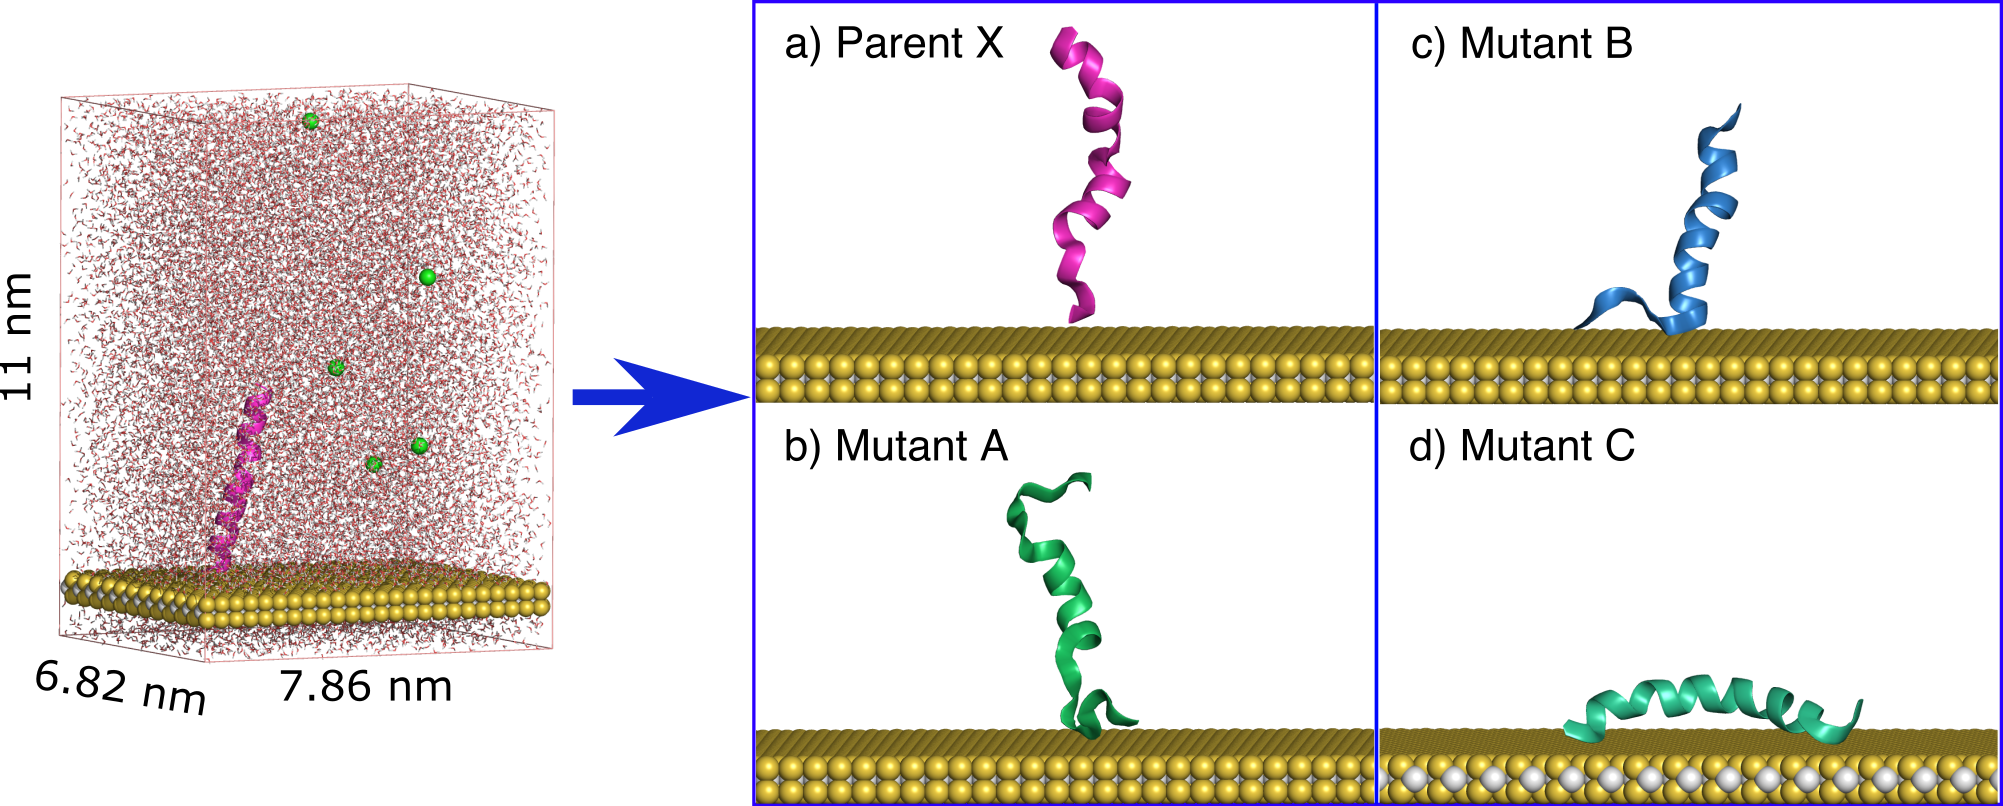
\includegraphics[width=\textwidth]{Tilting-simulation}
	\end{figure}
	\textcolor{blue}{$\Rightarrow$ the FF can reproduce experimental data}
\end{frame}


\begin{frame}
	\frametitle{Adsorption free energies of 20 naturally-occurring amino acids}
	\begin{figure}
		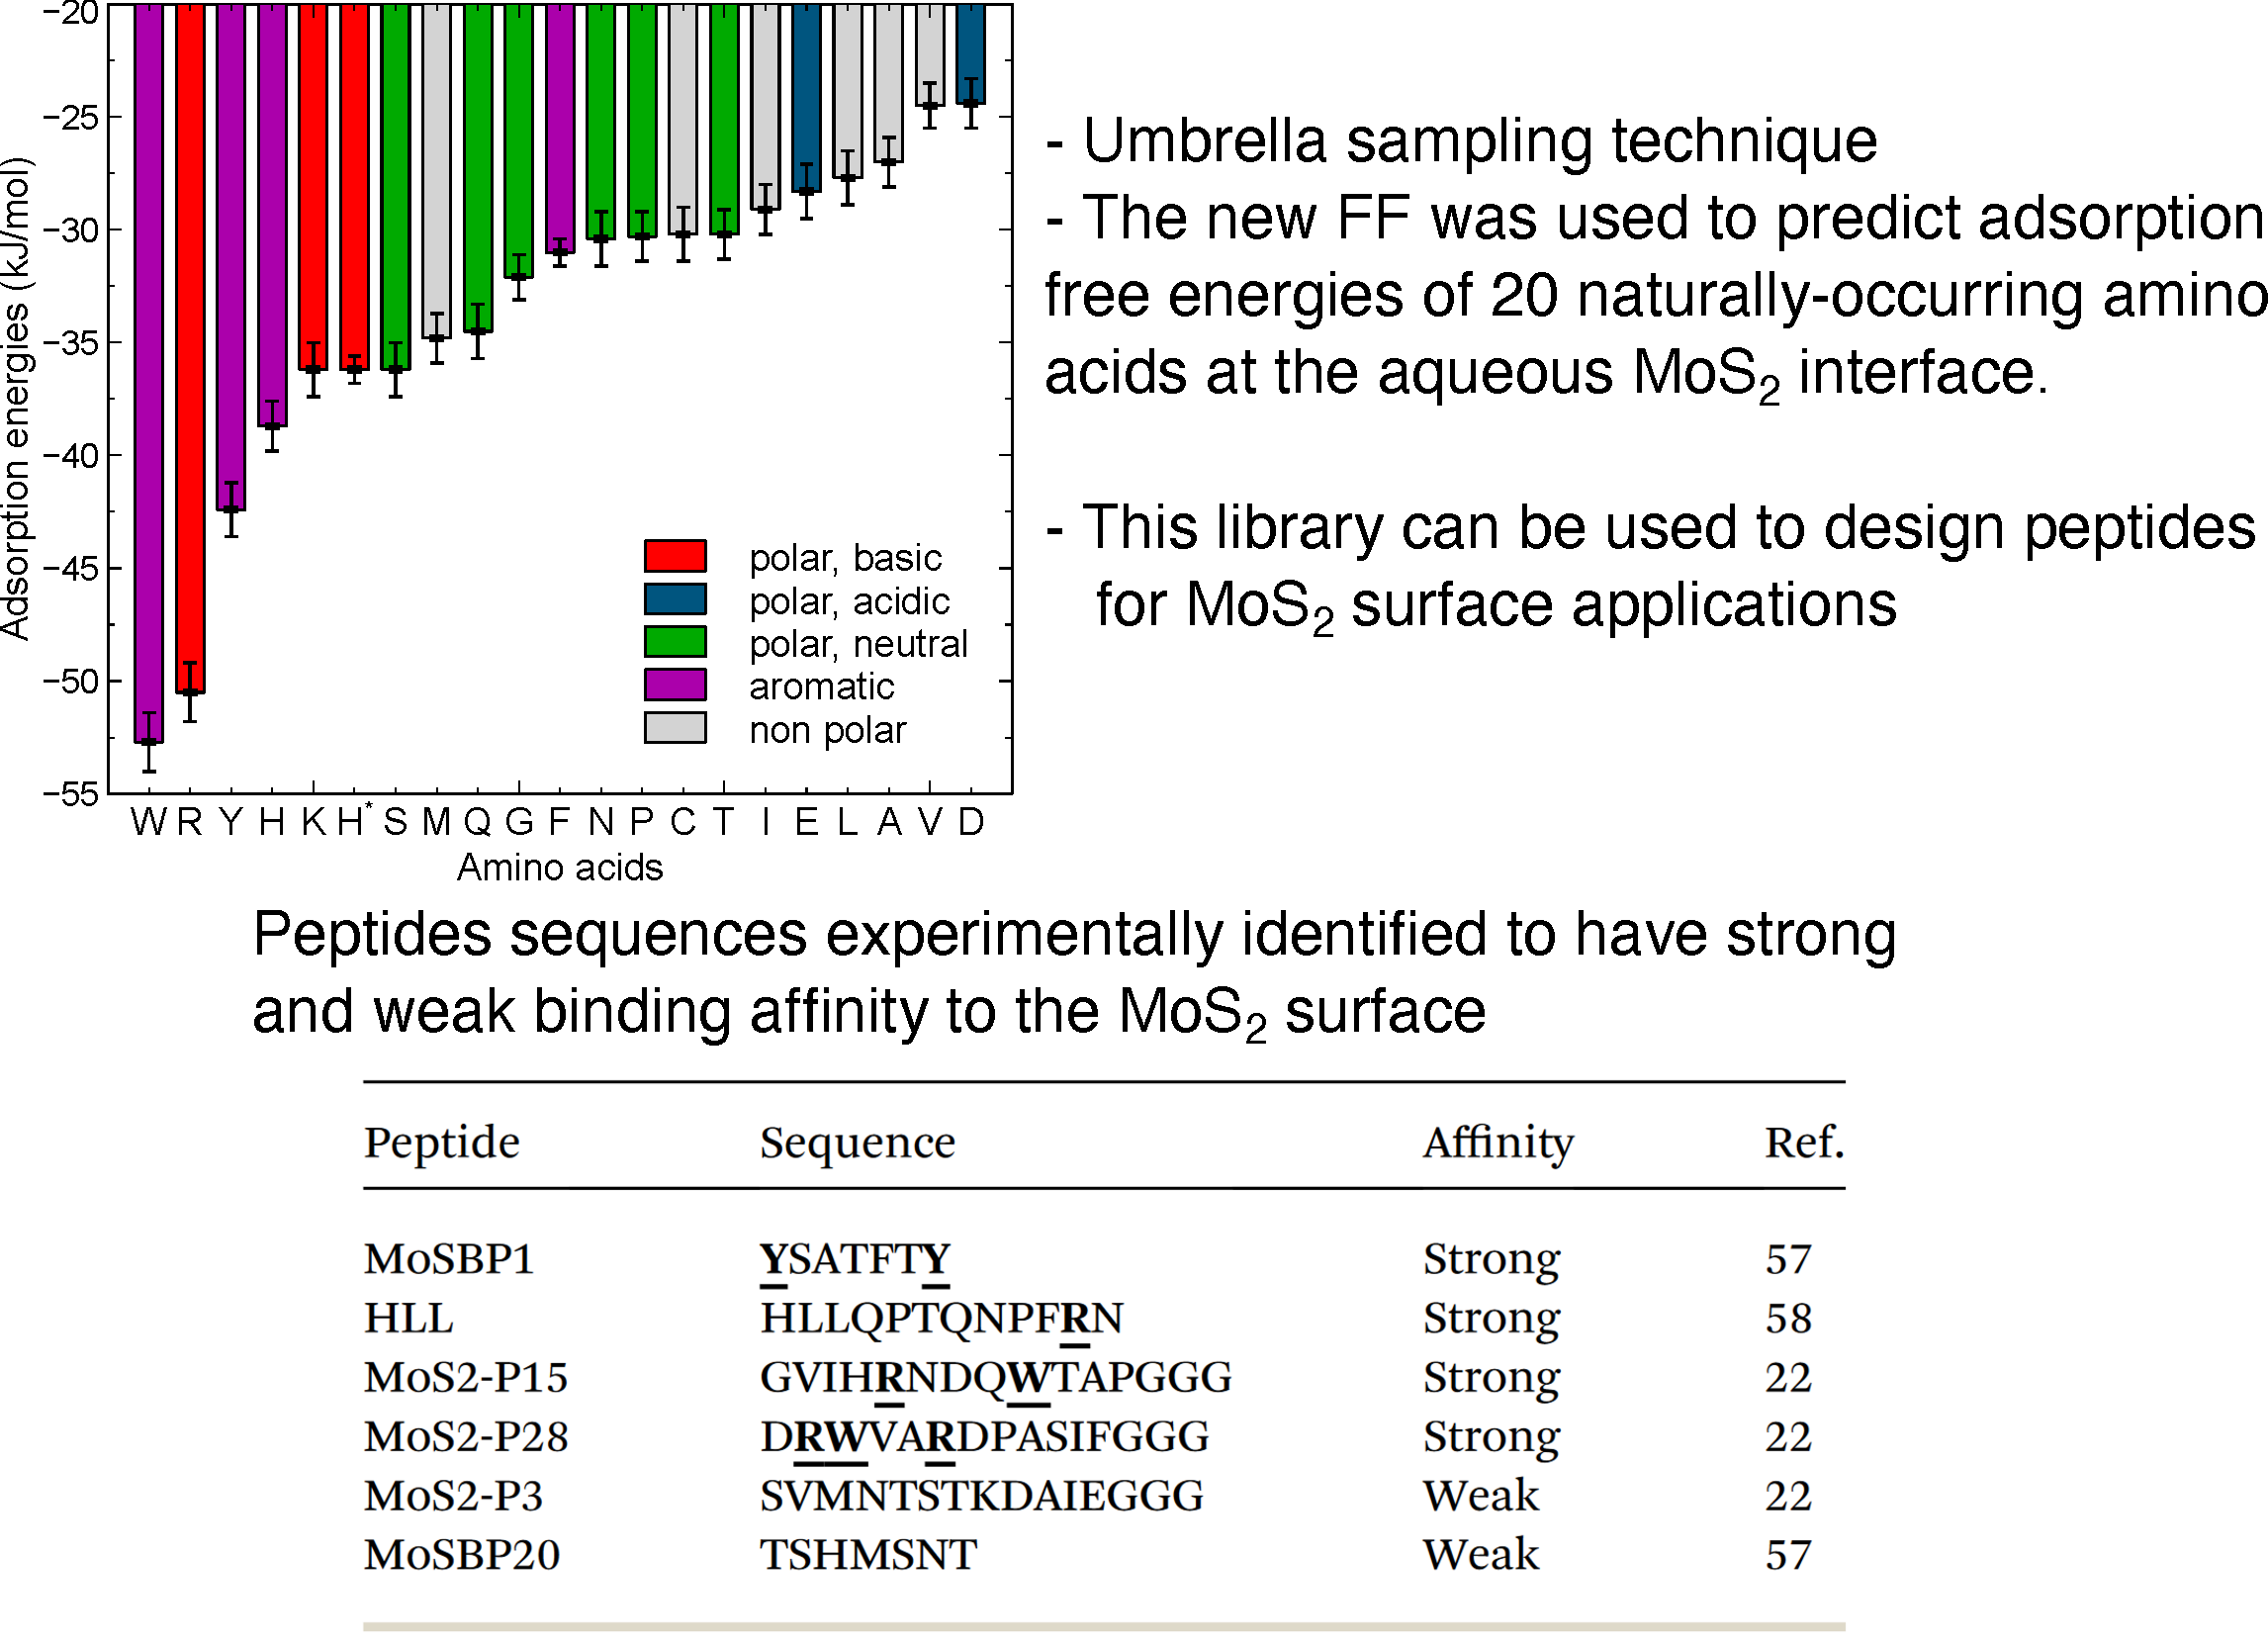
\includegraphics[height=0.9\textheight]{Firstapplication-FF}
	\end{figure}
\end{frame}


\begin{frame}
	\frametitle{Exfoliation of \ch{MoS2}: Simulation model design}
	\begin{figure}
		\includegraphics[width=0.75\textwidth]{2schemes.pdf}
	\end{figure}
	A video: https://twitter.com/LeNhanChem/status/1508950930624233474

\end{frame}

\begin{frame}
	\frametitle{Gap closing}
	\begin{figure}
		\includegraphics[width=0.55\textwidth]{exfoliationprocess}
	\end{figure}

\end{frame}



\begin{frame}
	\frametitle{Potential of Mean Force}
	\begin{figure}
		\includegraphics[width=\textwidth]{reachingPeptides-PFM}
	\end{figure}
	\tiny{Y.Perdomo,$^+$ L.N Pham,$^+$ T.R. Walsh and M.R.
		Knecht. \emph{Sustainable, Aqueous Exfoliation of \ch{MoS2} via Bio-Inspired Avenues.
			2023 (ready for submission) $^+$ equal contribution}}
\end{frame}


\section[3D crosslinked polymer matrices]{Optical properties of 3D crosslinked polymer matrices}

\begin{frame}
	\frametitle{3D crosslinked polymer matrices}
	\begin{figure}
		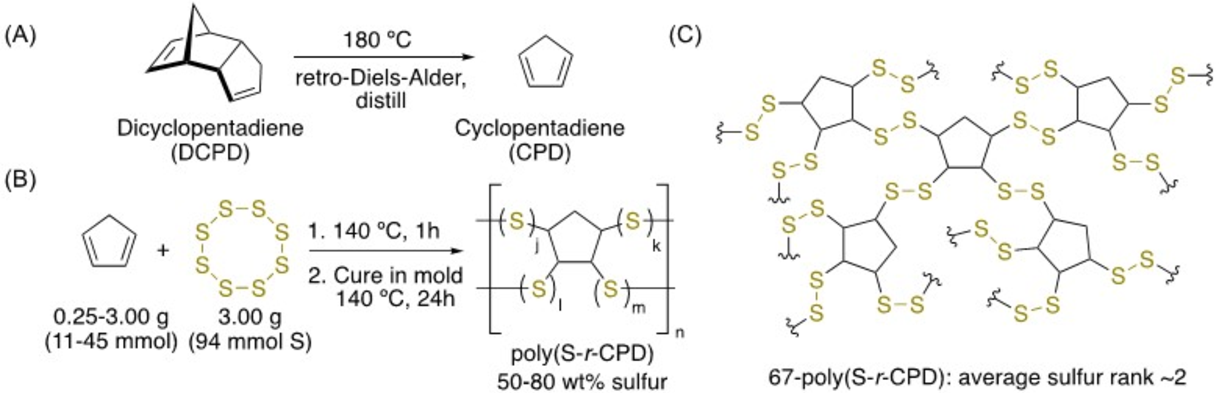
\includegraphics[width=0.7\textwidth]{3D-polymer-synthesis}
	\end{figure}
	\begin{itemize}
		\item IR inactive
		\item Potential applications: electronic devices, navigation of drones, autonomous vehicles, space exploration
		\item Which factors control optical properties and how to theoretically study them?
	\end{itemize}
	\tiny{Tonkin, S. J.; Pham, L. N.; Gascooke, J. R.; Johnston, M. R.; Coote, M. L.; Gibson, C. T.; Chalker, J. M.
		\emph{Thermal imaging and clandestine surveillance using low-cost polymers with long-wave infrared transparency} 10.26434/chemrxiv-2022-bzzd3}
\end{frame}


\begin{frame}
	\frametitle{Factors that can affect the optical properties}
	\begin{columns}
		\begin{column}{0.55\textwidth}
			\textcolor{blue}{Optical properties can be affected by:}
			%\vspace{-2cm}
			\begin{itemize}
				\item Cis and trans configurations of bridging atoms
				\item Size of the polymer
				\item 3D crosslinked architecture of the polymer
				\item Impurities in the polymer matrix: unsaturated bonds and other species
			\end{itemize}
		\end{column}
		\begin{column}{0.48\textwidth}
			\vspace{-0.2cm}
			\begin{figure}
				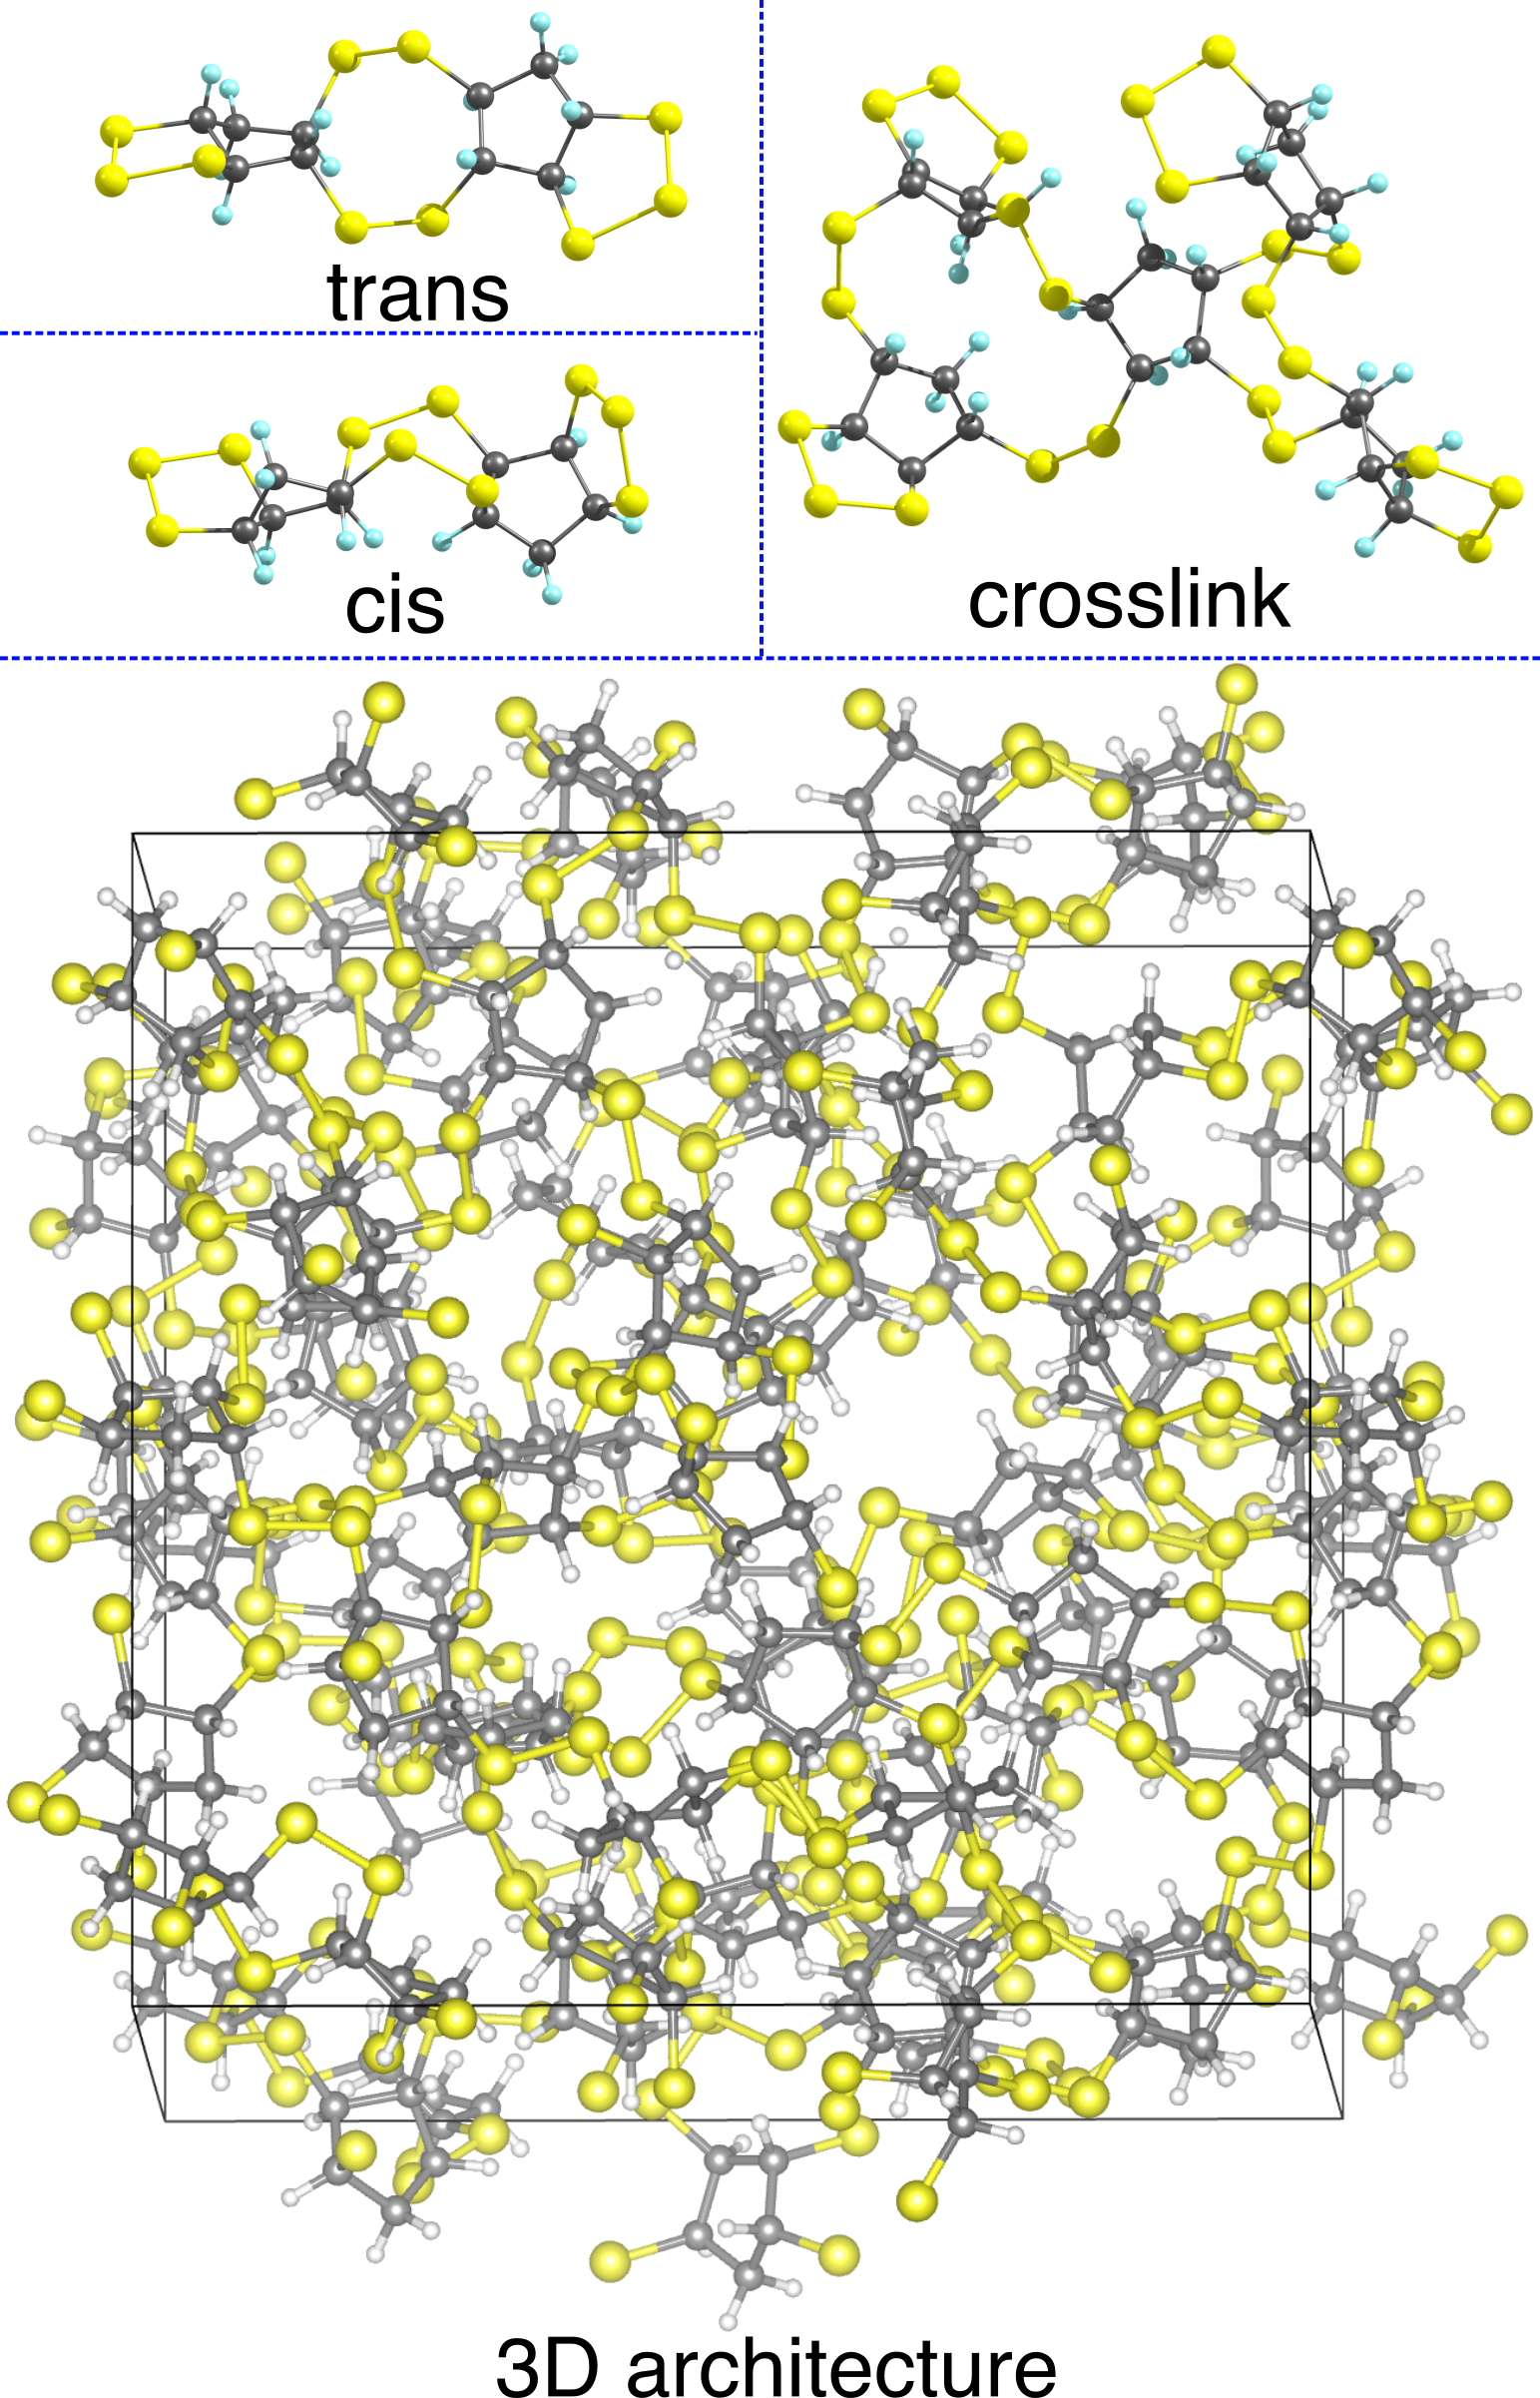
\includegraphics[height=0.88\textheight]{3-motifs}
			\end{figure}
		\end{column}
	\end{columns}
\end{frame}


\begin{frame}
	\frametitle{Construction of polymer models}
	\begin{itemize}
		\item Single chains: manual construction
		\item 3D crosslinked matrices: Use molecular dynamics to simulate pseudo reactions
	\end{itemize}
	\begin{figure}
		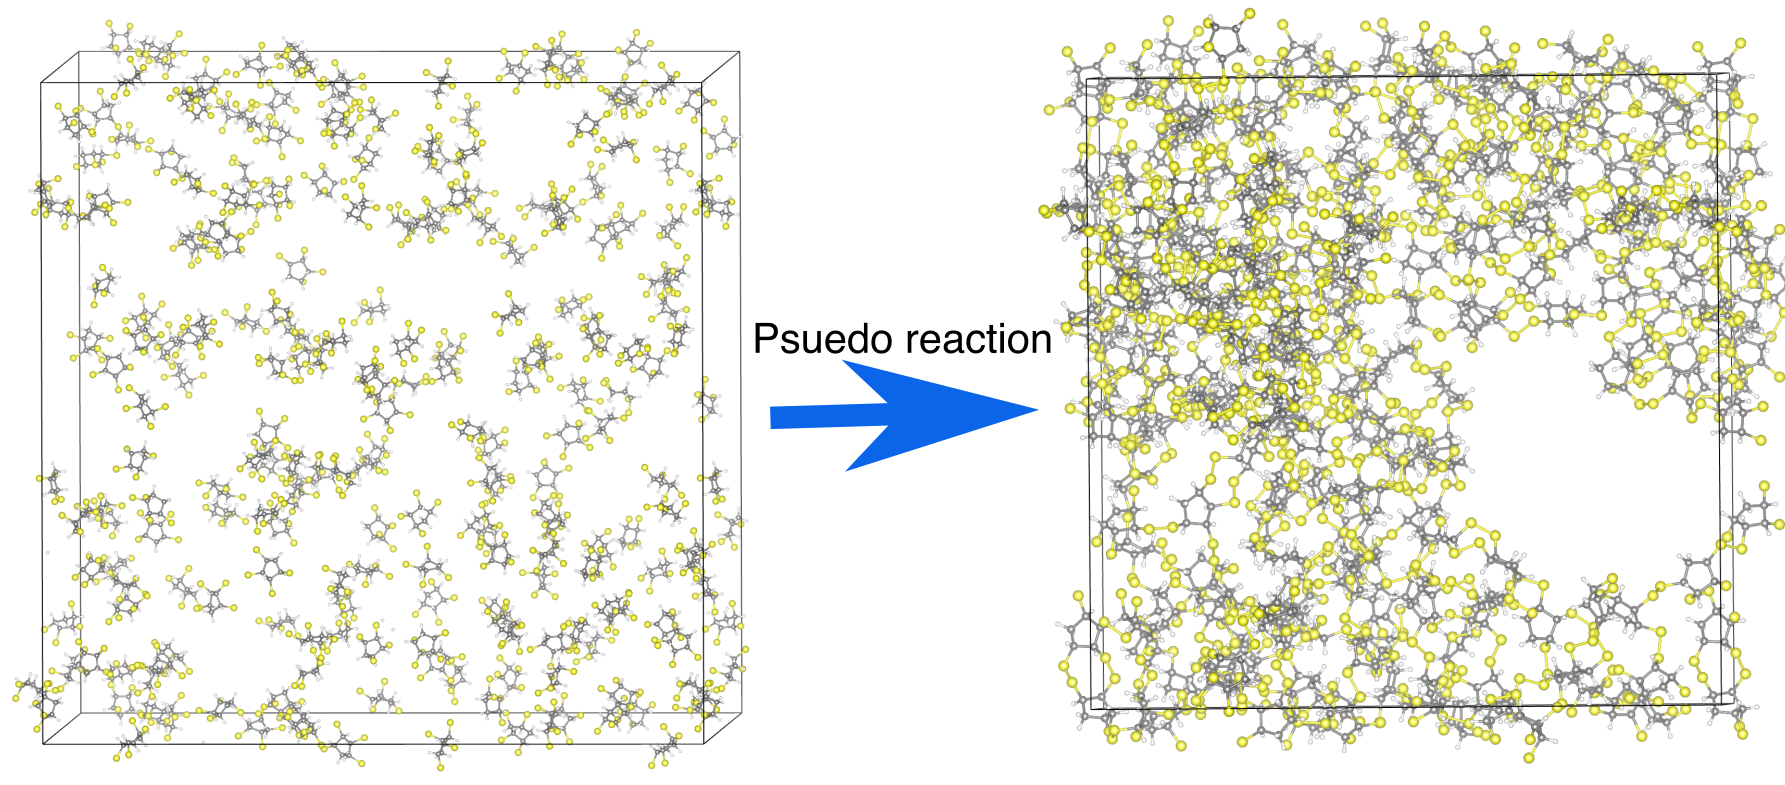
\includegraphics[width=0.85\textwidth]{Psuedo-reaction-polymerisation}
	\end{figure}

\end{frame}



\begin{frame}
	\frametitle{Convergence of IR spectra}
	\begin{figure}
		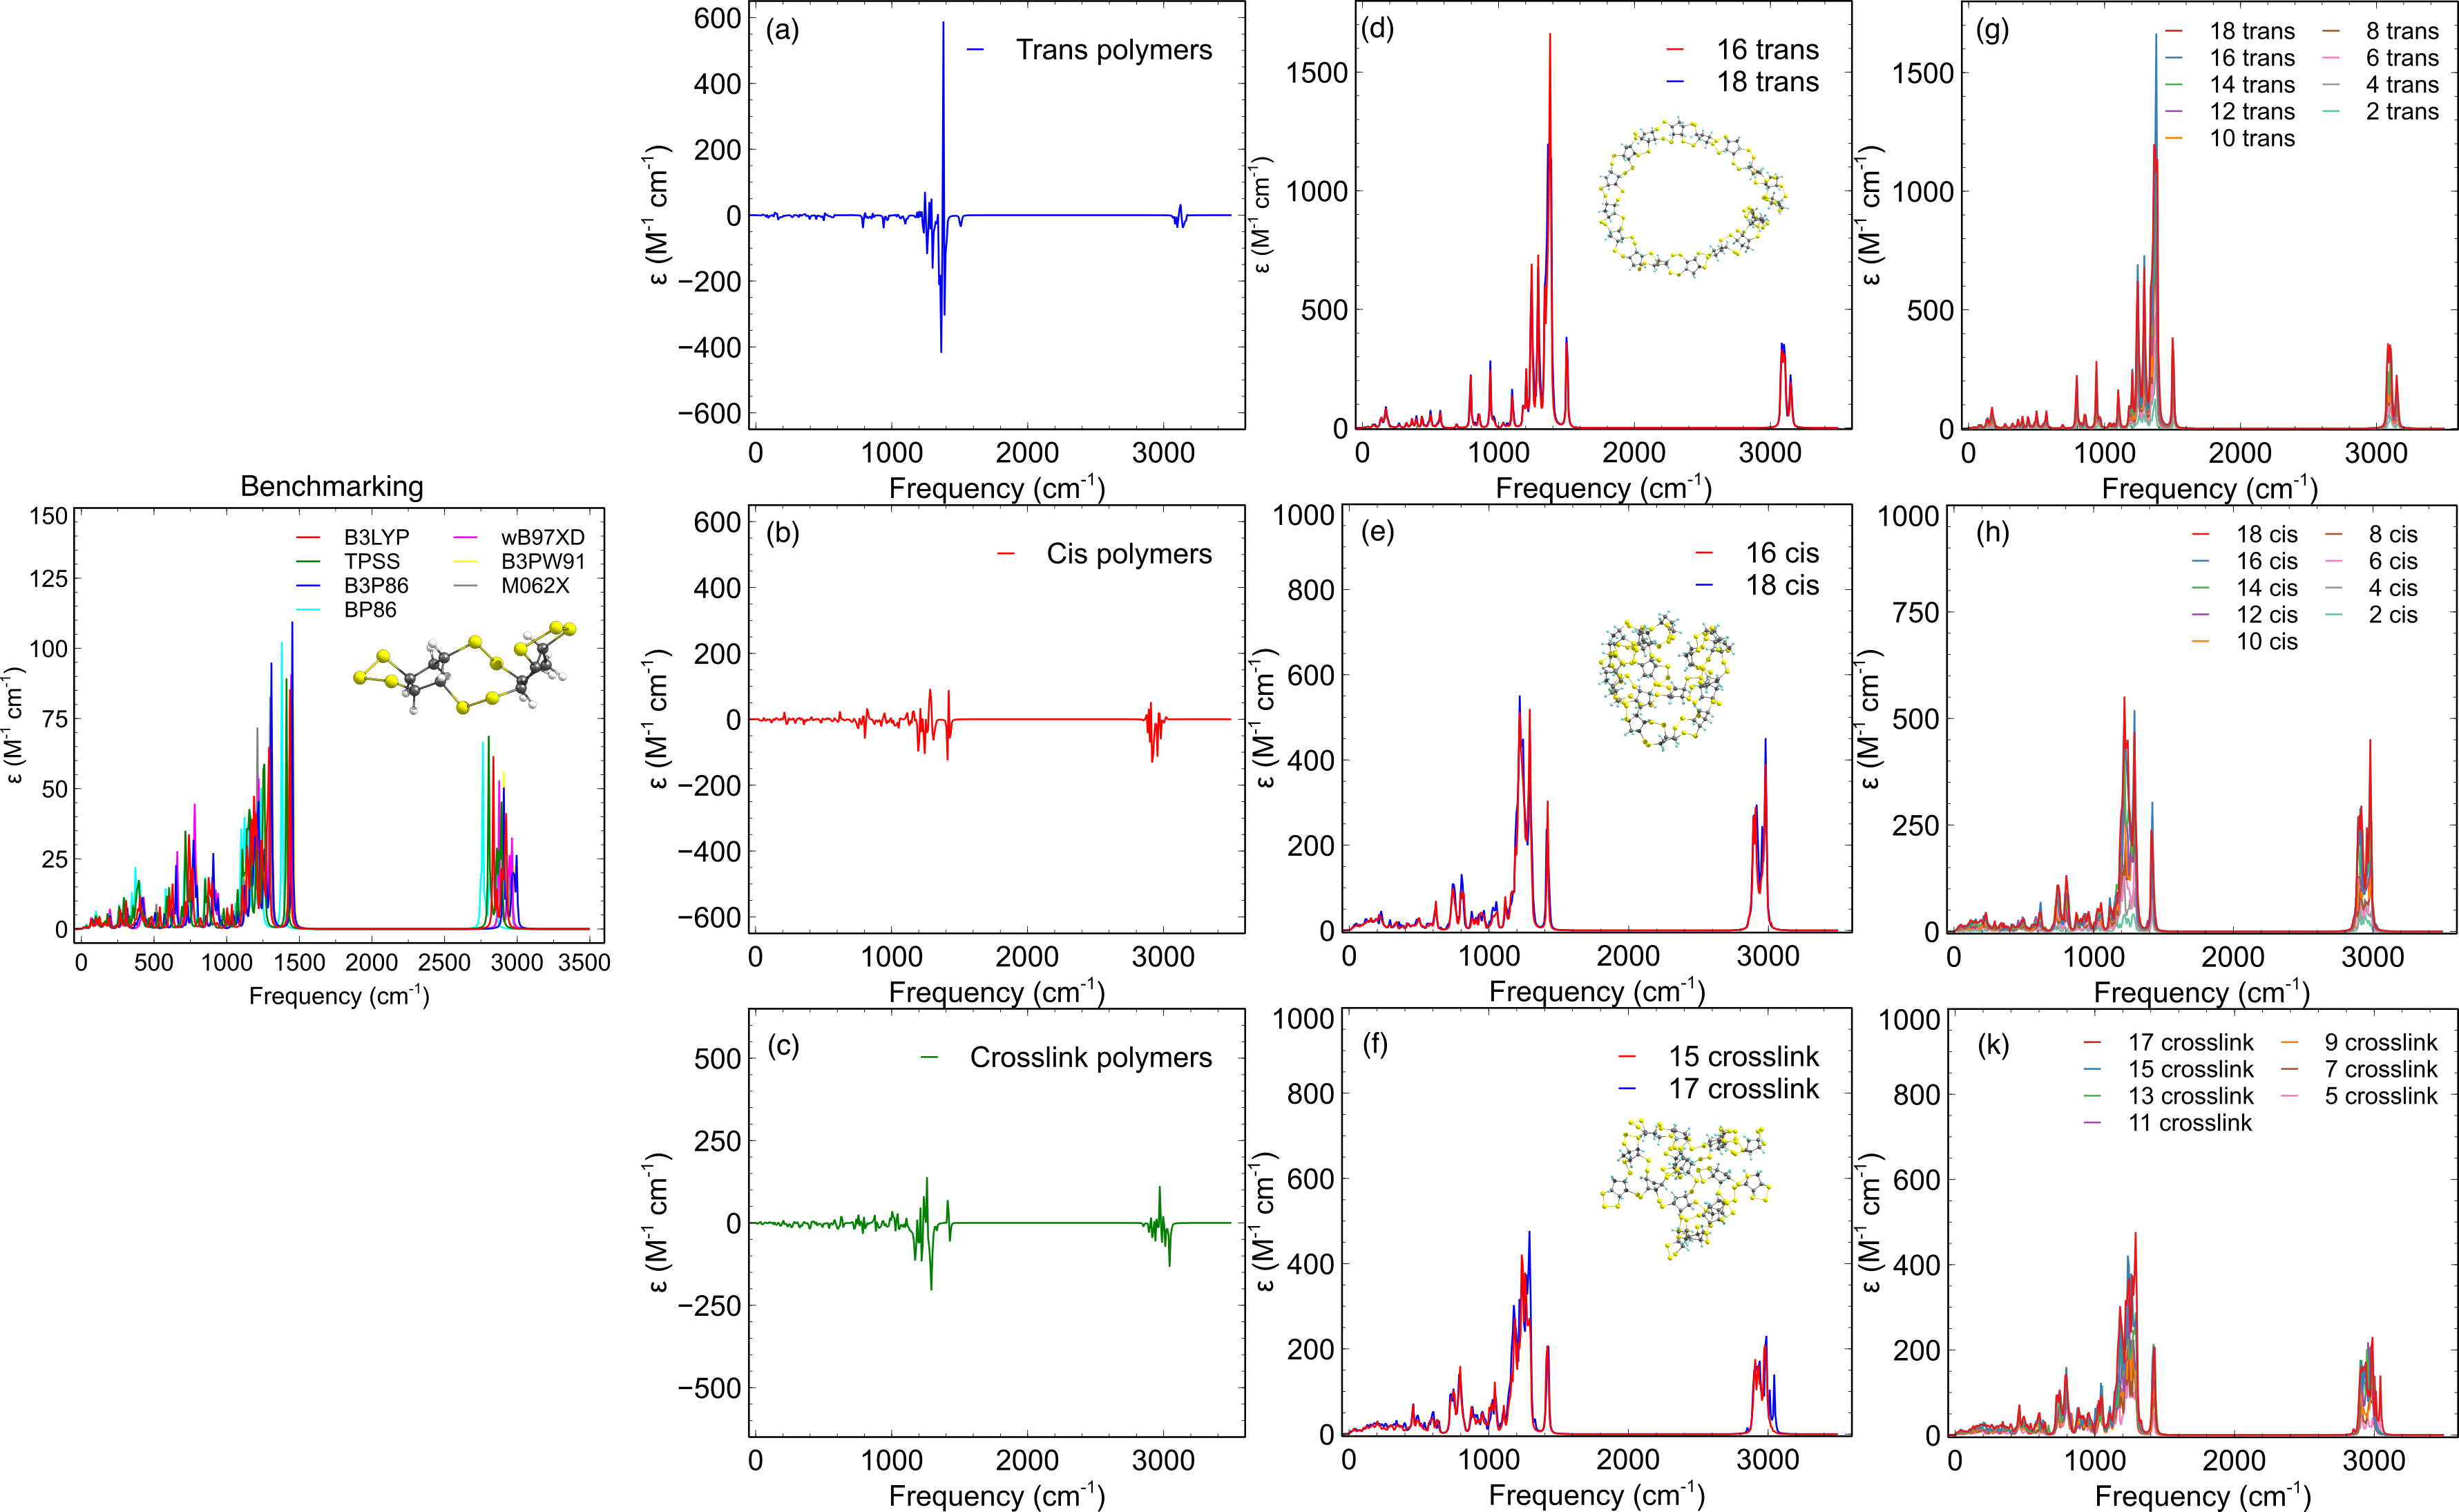
\includegraphics[height=0.89\textheight]{ChainLengthConvergence}
	\end{figure}
\end{frame}


\begin{frame}
	\frametitle{IR spectra of different motifs}
	\begin{figure}
		\includegraphics[height=0.89\textheight]{Diff-chemical-structures}
	\end{figure}
\end{frame}

\begin{frame}
	\frametitle{3D crosslinked architecture}
	\begin{columns}
		\begin{column}{0.5\textwidth}
			\begin{itemize}
				\item Rescaled vibrational frequencies of xTB
				\item Simulated IR spectra of 3D crosslinked polymer matrices at xTB level
				\item 3D crosslinked architecture does not affect optical properties
			\end{itemize}
		\end{column}
		\hspace{-1.5cm}
		\begin{column}{0.7\textwidth}
			\vspace{0.5mm}
			\begin{figure}
				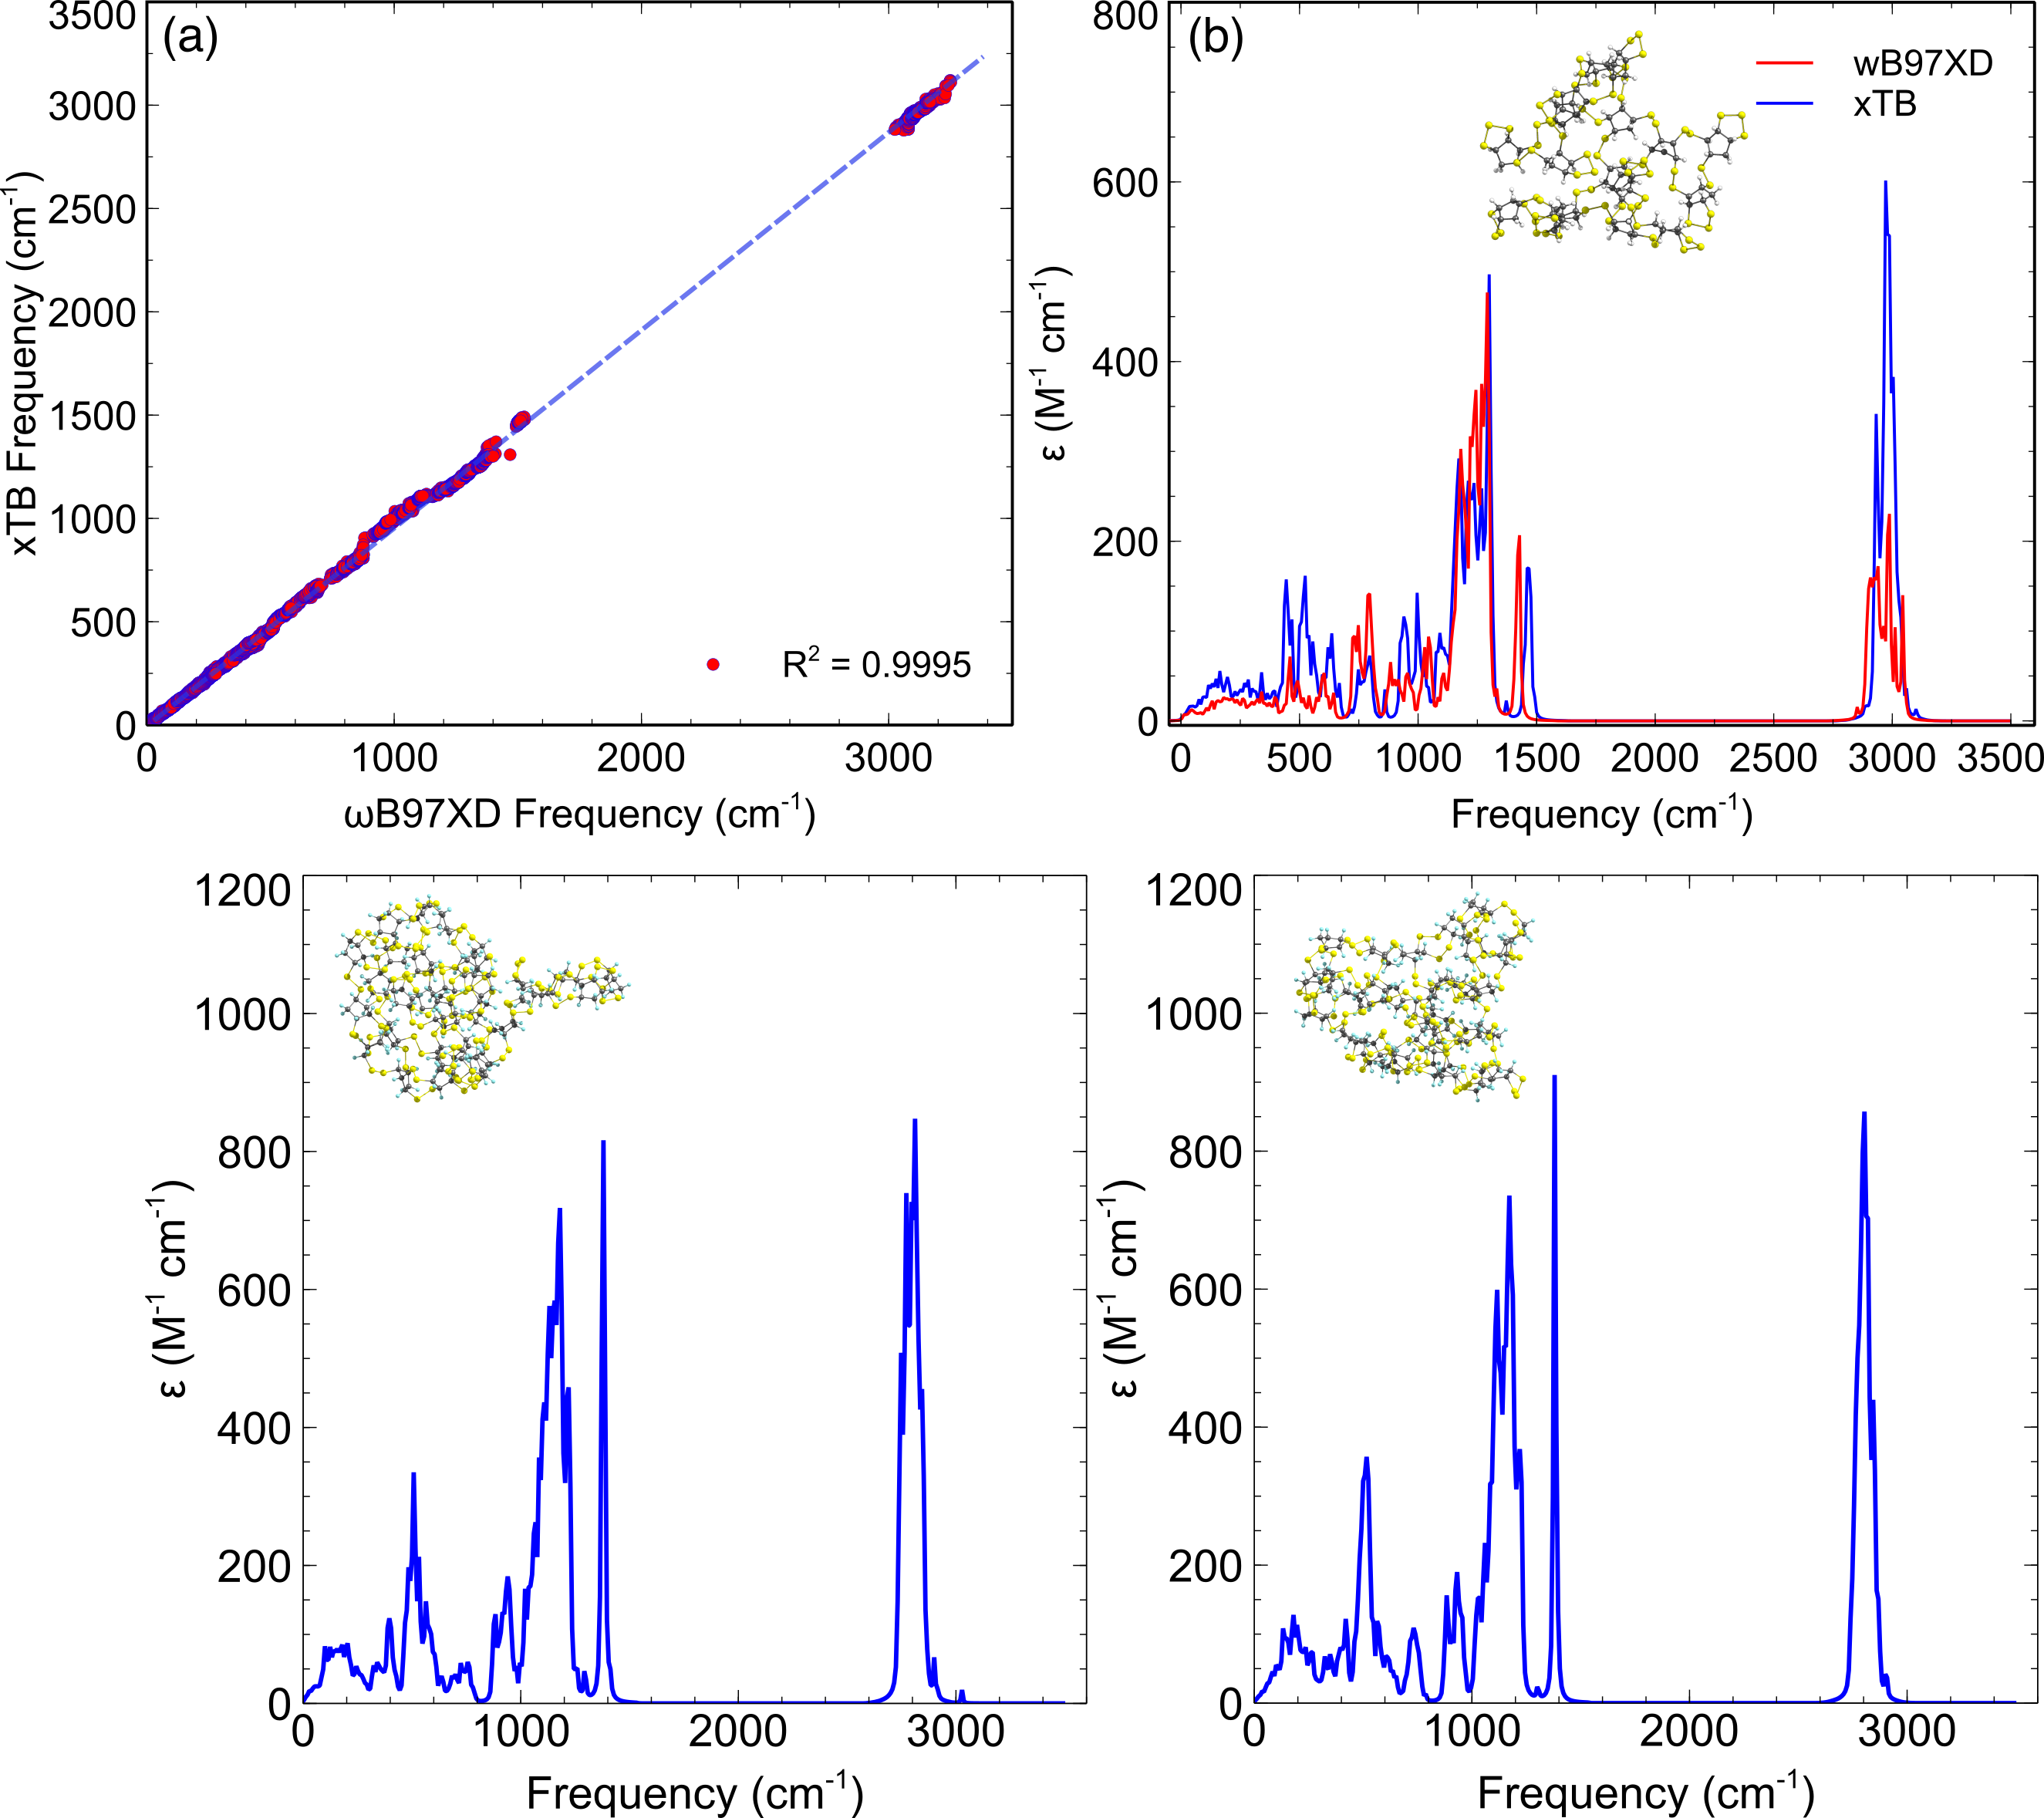
\includegraphics[height=0.85\textheight]{xTB-30-crosslink}
			\end{figure}
		\end{column}
	\end{columns}
\end{frame}

\begin{frame}
	\frametitle{Defects and impurities}
	\begin{figure}
		\includegraphics[width=0.95\textwidth]{Impurities}
	\end{figure}
\end{frame}

\begin{frame}
	\frametitle{Simulated vs Experiment}
	\begin{figure}
		\includegraphics[width=\textwidth]{Experimental-vs-Simulated-IR}
	\end{figure}
\end{frame}

\begin{frame}
	\frametitle{Final proposed IR spectrum}
	\begin{columns}
		\begin{column}{0.5\textwidth}
			\begin{itemize}
				\item Defects can affect optical properties of polymer matrices
				\item Other species may exist in the polymer matrices
				\item Polymer motifs (cis, trans), size, 3D architecture do not really affect optical properties
			\end{itemize}
		\end{column}
		\begin{column}{0.6\textwidth}
			\vspace{0.5mm}
			\begin{figure}
				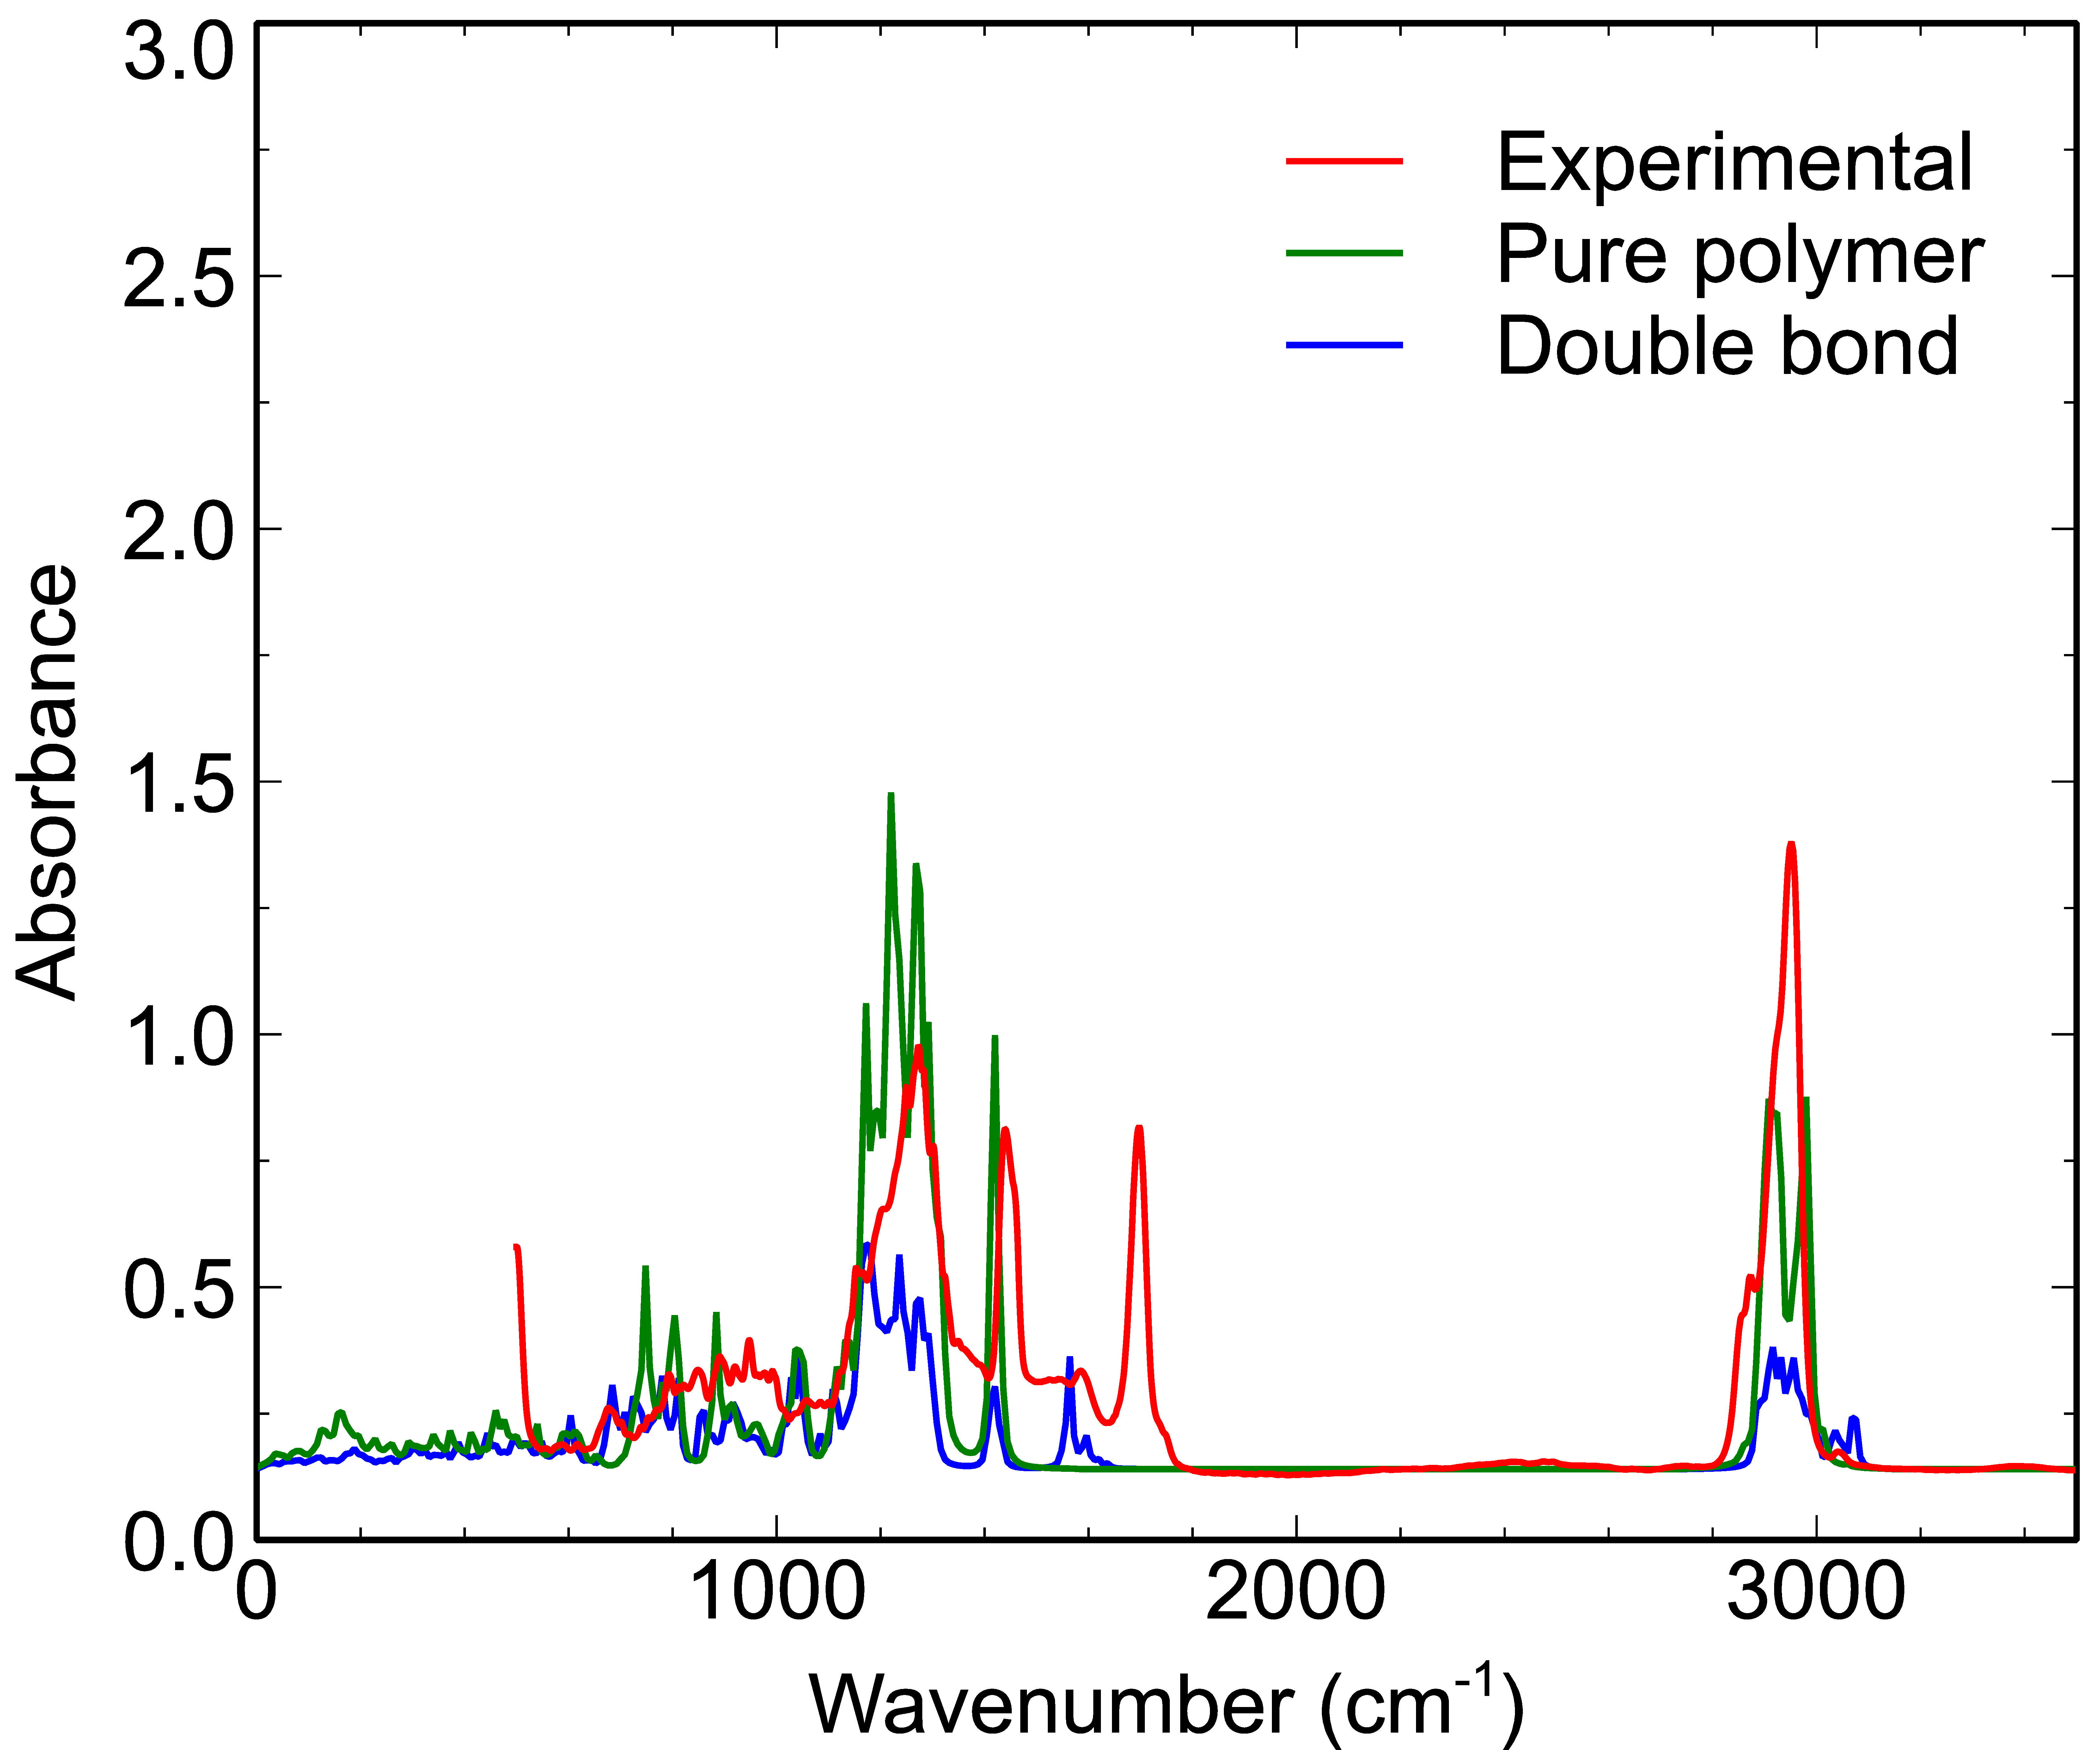
\includegraphics[height=0.75\textheight]{expt-vs-Average-simulated-spectra}
			\end{figure}
		\end{column}
	\end{columns}
\end{frame}



\section{Conclusion}

\begin{frame}
	\frametitle{Conclusion}
	\textcolor{blue}{QM and MD methods have been used to support each other in study of complicated systems}
	\begin{itemize}
		\item A procedure introduced to evaluate and benchmark FFs based on quantum chemical data 
		\item A high-accuracy FF was developed based on quantum chemical data
		\item MD simulations were used to construct complicated systems for further QM calculations
	\end{itemize}
\end{frame}


\begin{frame}
	\frametitle{Thank you}
	We want to thank:
	\begin{figure}
		\includegraphics[width=0.5\textwidth]{logo}
	\end{figure}
	\begin{itemize}
		\item Specially grateful to Prof. Tiffany Walsh (Deakin Uni) and Prof. Michelle Coote (Flinders Uni) for their excellent scientific guidance
		\item The APATCC-10 organizers for huge efforts and energy to organize this conference
	\end{itemize}
\end{frame}






%%%%%%%%%%%%%%%%%%%%%%%%%%%%%

\subsection*{Thank you}

\begin{frame}{Thank you for your attention}
	\centering
	\textcolor{flinders-blue}{\textbf{\LARGE Thank you for your attention}}\\

	\vspace{0.5cm}

	\begin{CJK*}{UTF8}{zhsong}
		\textcolor{red}{\textbf{\LARGE 多谢}} \clearpage\end{CJK*}

	\textcolor{kul-blue}{\textbf{\LARGE CẢM ƠN}}\\

\end{frame}


\end{document}
